% Options for packages loaded elsewhere
\PassOptionsToPackage{unicode}{hyperref}
\PassOptionsToPackage{hyphens}{url}
%
\documentclass[
  letterpaper,
  DIV=11,
  numbers=noendperiod]{scrartcl}

\usepackage{amsmath,amssymb}
\usepackage{setspace}
\usepackage{iftex}
\ifPDFTeX
  \usepackage[T1]{fontenc}
  \usepackage[utf8]{inputenc}
  \usepackage{textcomp} % provide euro and other symbols
\else % if luatex or xetex
  \usepackage{unicode-math}
  \defaultfontfeatures{Scale=MatchLowercase}
  \defaultfontfeatures[\rmfamily]{Ligatures=TeX,Scale=1}
\fi
\usepackage{lmodern}
\ifPDFTeX\else  
    % xetex/luatex font selection
\fi
% Use upquote if available, for straight quotes in verbatim environments
\IfFileExists{upquote.sty}{\usepackage{upquote}}{}
\IfFileExists{microtype.sty}{% use microtype if available
  \usepackage[]{microtype}
  \UseMicrotypeSet[protrusion]{basicmath} % disable protrusion for tt fonts
}{}
\makeatletter
\@ifundefined{KOMAClassName}{% if non-KOMA class
  \IfFileExists{parskip.sty}{%
    \usepackage{parskip}
  }{% else
    \setlength{\parindent}{0pt}
    \setlength{\parskip}{6pt plus 2pt minus 1pt}}
}{% if KOMA class
  \KOMAoptions{parskip=half}}
\makeatother
\usepackage{xcolor}
\setlength{\emergencystretch}{3em} % prevent overfull lines
\setcounter{secnumdepth}{5}
% Make \paragraph and \subparagraph free-standing
\makeatletter
\ifx\paragraph\undefined\else
  \let\oldparagraph\paragraph
  \renewcommand{\paragraph}{
    \@ifstar
      \xxxParagraphStar
      \xxxParagraphNoStar
  }
  \newcommand{\xxxParagraphStar}[1]{\oldparagraph*{#1}\mbox{}}
  \newcommand{\xxxParagraphNoStar}[1]{\oldparagraph{#1}\mbox{}}
\fi
\ifx\subparagraph\undefined\else
  \let\oldsubparagraph\subparagraph
  \renewcommand{\subparagraph}{
    \@ifstar
      \xxxSubParagraphStar
      \xxxSubParagraphNoStar
  }
  \newcommand{\xxxSubParagraphStar}[1]{\oldsubparagraph*{#1}\mbox{}}
  \newcommand{\xxxSubParagraphNoStar}[1]{\oldsubparagraph{#1}\mbox{}}
\fi
\makeatother


\providecommand{\tightlist}{%
  \setlength{\itemsep}{0pt}\setlength{\parskip}{0pt}}\usepackage{longtable,booktabs,array}
\usepackage{calc} % for calculating minipage widths
% Correct order of tables after \paragraph or \subparagraph
\usepackage{etoolbox}
\makeatletter
\patchcmd\longtable{\par}{\if@noskipsec\mbox{}\fi\par}{}{}
\makeatother
% Allow footnotes in longtable head/foot
\IfFileExists{footnotehyper.sty}{\usepackage{footnotehyper}}{\usepackage{footnote}}
\makesavenoteenv{longtable}
\usepackage{graphicx}
\makeatletter
\def\maxwidth{\ifdim\Gin@nat@width>\linewidth\linewidth\else\Gin@nat@width\fi}
\def\maxheight{\ifdim\Gin@nat@height>\textheight\textheight\else\Gin@nat@height\fi}
\makeatother
% Scale images if necessary, so that they will not overflow the page
% margins by default, and it is still possible to overwrite the defaults
% using explicit options in \includegraphics[width, height, ...]{}
\setkeys{Gin}{width=\maxwidth,height=\maxheight,keepaspectratio}
% Set default figure placement to htbp
\makeatletter
\def\fps@figure{htbp}
\makeatother
% definitions for citeproc citations
\NewDocumentCommand\citeproctext{}{}
\NewDocumentCommand\citeproc{mm}{%
  \begingroup\def\citeproctext{#2}\cite{#1}\endgroup}
\makeatletter
 % allow citations to break across lines
 \let\@cite@ofmt\@firstofone
 % avoid brackets around text for \cite:
 \def\@biblabel#1{}
 \def\@cite#1#2{{#1\if@tempswa , #2\fi}}
\makeatother
\newlength{\cslhangindent}
\setlength{\cslhangindent}{1.5em}
\newlength{\csllabelwidth}
\setlength{\csllabelwidth}{3em}
\newenvironment{CSLReferences}[2] % #1 hanging-indent, #2 entry-spacing
 {\begin{list}{}{%
  \setlength{\itemindent}{0pt}
  \setlength{\leftmargin}{0pt}
  \setlength{\parsep}{0pt}
  % turn on hanging indent if param 1 is 1
  \ifodd #1
   \setlength{\leftmargin}{\cslhangindent}
   \setlength{\itemindent}{-1\cslhangindent}
  \fi
  % set entry spacing
  \setlength{\itemsep}{#2\baselineskip}}}
 {\end{list}}
\usepackage{calc}
\newcommand{\CSLBlock}[1]{\hfill\break\parbox[t]{\linewidth}{\strut\ignorespaces#1\strut}}
\newcommand{\CSLLeftMargin}[1]{\parbox[t]{\csllabelwidth}{\strut#1\strut}}
\newcommand{\CSLRightInline}[1]{\parbox[t]{\linewidth - \csllabelwidth}{\strut#1\strut}}
\newcommand{\CSLIndent}[1]{\hspace{\cslhangindent}#1}

\usepackage{booktabs}
\usepackage{caption}
\usepackage{longtable}
\usepackage{colortbl}
\usepackage{array}
\usepackage{anyfontsize}
\usepackage{multirow}
\KOMAoption{captions}{tableheading}
\usepackage[left]{lineno}
\linenumbers
\usepackage{xcolor}
\usepackage{float}
\floatplacement{table}{H}
\usepackage{setspace}
\makeatletter
\@ifpackageloaded{caption}{}{\usepackage{caption}}
\AtBeginDocument{%
\ifdefined\contentsname
  \renewcommand*\contentsname{Table of contents}
\else
  \newcommand\contentsname{Table of contents}
\fi
\ifdefined\listfigurename
  \renewcommand*\listfigurename{List of Figures}
\else
  \newcommand\listfigurename{List of Figures}
\fi
\ifdefined\listtablename
  \renewcommand*\listtablename{List of Tables}
\else
  \newcommand\listtablename{List of Tables}
\fi
\ifdefined\figurename
  \renewcommand*\figurename{Figure}
\else
  \newcommand\figurename{Figure}
\fi
\ifdefined\tablename
  \renewcommand*\tablename{Table}
\else
  \newcommand\tablename{Table}
\fi
}
\@ifpackageloaded{float}{}{\usepackage{float}}
\floatstyle{ruled}
\@ifundefined{c@chapter}{\newfloat{codelisting}{h}{lop}}{\newfloat{codelisting}{h}{lop}[chapter]}
\floatname{codelisting}{Listing}
\newcommand*\listoflistings{\listof{codelisting}{List of Listings}}
\makeatother
\makeatletter
\makeatother
\makeatletter
\@ifpackageloaded{caption}{}{\usepackage{caption}}
\@ifpackageloaded{subcaption}{}{\usepackage{subcaption}}
\makeatother

\ifLuaTeX
  \usepackage{selnolig}  % disable illegal ligatures
\fi
\usepackage{bookmark}

\IfFileExists{xurl.sty}{\usepackage{xurl}}{} % add URL line breaks if available
\urlstyle{same} % disable monospaced font for URLs
\hypersetup{
  pdftitle={Snow Interception Relationships with Meteorology and Canopy Density in a Subalpine Forest},
  hidelinks,
  pdfcreator={LaTeX via pandoc}}


\title{Snow Interception Relationships with Meteorology and Canopy
Density in a Subalpine Forest}
\author{}
\date{}

\begin{document}
\maketitle


\setstretch{1.5}
\setstretch{1.5}

\textbf{Authors:}

Alex C. Cebulski\textsuperscript{1} (ORCID ID - 0000-0001-7910-5056)

John W. Pomeroy\textsuperscript{1} (ORCID ID - 0000-0002-4782-7457)

\textsuperscript{1}Centre for Hydrology, University of Saskatchewan,
Canmore, Canada

\textbf{Corresponding Author:} A.C. Cebulski, alex.cebulski@usask.ca

\textbf{Abstract:} Snow accumulation models differ in how snow
interception and ablation processes are represented and thus their
application to diverse climates and forest types is uncertain. Existing
parameterisations of initial snow interception before unloading include
inherently coupled canopy snow accumulation and ablation processes. This
leads to difficulty in diagnosing processes and adding possible errors
to simulations when incorporated as canopy interception routines in
models that already account for canopy snow ablation. This study
evaluates the theory underpinning parameterisations of initial snow
interception using high-temporal resolution and fine-scale measurements
of throughfall for events with minimal snow ablation and redistribution
in both the canopy and on the ground. Relationships between these
throughfall measurements, event meteorology, and a novel lidar-based
canopy density measurement were assessed in two subalpine forest plots
in the Canadian Rockies. Contrary to existing theories, no association
of canopy snow load or air temperature with interception efficiency was
observed. Instead, snow-leaf contact area emerged as the primary factor
governing snow accumulation. A wind-driven snowfall event demonstrated
that non-vertical hydrometeor trajectories can significantly increase
snow-leaf contact area, thereby enhancing initial interception before
ablation. Prediction of interception efficiency for this event was
improved when adjusted for hydrometeor trajectory angle based on the
wind speed at one-third of the canopy height. Snow-leaf contact area
showed a high sensitivity to wind speed, increasing by up to 95\% with a
1 m s\textsuperscript{-1} wind speed. The study proposes a new
parameterisation that calculates throughfall, independent of processes
that ablate snow from the canopy, as a function of snowfall, canopy
cover, wind speed, and hydrometeor fall velocity. This new
parameterisation successfully estimated subcanopy snow accumulation for
a snowfall event at two forest plots of differing canopy density and
structure. By separating canopy snow ablation from snow interception
processes, this new model offers potentially improved prediction of
subcanopy snow accumulation when combined with canopy snow ablation
parameterisations.

\textbf{Keywords:} snow interception, throughfall, ablation, forest,
snowpack, lidar, process-based modelling

\section{Introduction}\label{introduction}

Over half of North America's snow-covered zone is covered by forests
(Kim et al., 2017), significantly impacting the accumulation and
redistribution of snowpacks and subsequent snowmelt runoff. Essery et
al. (2003) estimated that 25--45\% of annual snowfall may be lost to the
atmosphere due to sublimation of snow intercepted in forest canopies
globally. Snow intercepted in the canopy can sublimate and melt at much
higher rates than the subcanopy snowpack (Katsushima et al., 2023;
Lundberg \& Halldin, 1994; Pomeroy et al., 1998), reducing the amount of
snow available for runoff. Canopy density is one of the primary factors
controlling the partitioning of snowfall into throughfall and
interception (Hedstrom \& Pomeroy, 1998; Staines \& Pomeroy, 2023) and
thus governs the quantity of snow subject to sublimation from the
canopy. Canopy structure metrics such as distance to canopy edge and
total gap area have also shown strong correlations to throughfall
measurements at the event-based (Moeser et al., 2015a) and seasonal
(Mazzotti et al., 2019) timescales. Despite these relationships, forest
thinning efforts aimed at limiting sublimation losses to increase
snowmelt runoff do not always lead to a corresponding increase in spring
streamflow (Golding \& Swanson, 1978; Harpold et al., 2020; Pomeroy et
al., 2012; Troendle, 1983). This may be due to increased ablation rates
when forest cover is reduced, desynchronization of snowmelt timing, and
sub-surface hydrology interactions (Ellis et al., 2013; Musselman et
al., 2015; Pomeroy et al., 1997; Safa et al., 2021; Varhola et al.,
2010). Given the significant impact of forest cover on snowpacks, along
with the limited or absent monitoring networks for subcanopy snow
accumulation (Rittger et al., 2020; Vionnet et al., 2021), land
management, ecological conservation, and water resource decisions depend
on reliable models of snow redistribution.

Hedstrom \& Pomeroy (1998), working in the cold continental boreal
forest, proposed that initial snow interception efficiency was
controlled by the maximum canopy load which itself was a function of
leaf area index and fresh snow density. Andreadis et al. (2009),
incorporating measurements from several studies (Kobayashi, 1987;
Pfister \& Schneebeli, 1999; Storck et al., 2002), emphasized the role
of leaf area index and air temperature in controlling the maximum canopy
snow load. Although these two parameterisations incorporate different
processes and relationships with air temperature, the Hedstrom \&
Pomeroy (1998) initial snow interception parameterisation has shown
strong performance at sites across Canada, Russia, Switzerland, and
Spain (Ellis et al., 2010; Gelfan et al., 2004; Pomeroy et al., 2022;
Sanmiguel-Vallelado et al., 2022), while the Andreadis et al. (2009)
parameterisation has produced accurate results in coastal environments
(Andreadis et al., 2009; Clark et al., 2015). Subsequent research by
Lundquist et al. (2021) and Lumbrazo et al. (2022) has revealed
overestimation of subcanopy snow accumulation when combining the
Hedstrom \& Pomeroy (1998) routine with ablation parameterisations from
different studies (i.e., Roesch et al., 2001). The coupling of ablation
processes within existing snow interception parameterisations (Andreadis
et al., 2009; Hedstrom \& Pomeroy, 1998) may contribute to overestimates
of throughfall, canopy snow unloading, and canopy snowmelt when combined
with other canopy snow ablation parameterisations (Cebulski \& Pomeroy,
2025). Additional observations that separate initial snow interception
from ablation processes could help determine the applicability of the
interception theories proposed by Hedstrom \& Pomeroy (1998) and
Andreadis et al. (2009). Hedstrom \& Pomeroy's (1998) theory also
suggests that moderate wind speeds, which can result in more horizontal
hydrometeor trajectories, increasing snow-leaf contact area and
interception efficiency at the plot scale. This association has also
been shown in rainfall interception studies to decrease throughfall of
rain (Herwitz \& Slye, 1995; Van Stan et al., 2011). However, the
relationship proposed by Hedstrom \& Pomeroy (1998), is typically not
included in snow accumulation models as empirical testing of this
relationship is lacking.

The objective of this paper is to evaluate the theories underlying
existing snow interception models using high spatial and temporal
resolution measurements of subcanopy snow accumulation for events with
minimal canopy snow ablation. These new observations are investigated to
address the following research questions:

\begin{enumerate}
\def\labelenumi{\arabic{enumi}.}
\item
  Are the existing theories regarding the relationships between
  meteorology and canopy density and initial snow interception supported
  by in-situ observations collected in the Canadian Rockies?
\item
  How is initial snow interception influenced by non-vertical
  hydrometeor trajectory angles over a wind-driven snowfall event?
\item
  To what extent can these findings inform the development of a new
  parameterisation for initial snow interception?
\end{enumerate}

\section{Theory}\label{theory}

\subsection{Canopy snow mass balance}\label{canopy-snow-mass-balance}

The change in canopy snow load over time, \(\frac{dL}{dt}\) (mm
s\textsuperscript{-1}), can be estimated from the mass balance:

\begin{equation}\phantomsection\label{eq-canopy-mass-bal}{
\frac{dL}{dt} = 
[q_{sf} - q_{tf} + q_{ros}] - q_{unld} - q_{drip} - q_{wind}^{veg} - q_{sub}^{veg}
}\end{equation}

where \(q_{sf}\) is the snowfall rate (mm s\textsuperscript{-1}),
\(q_{tf}\) (mm s\textsuperscript{-1}) is the throughfall rate (mm
s\textsuperscript{-1}), \(q_{ros}\) (mm s\textsuperscript{-1}) is the
rate of rainfall falling on snow intercepted in the canopy, \(q_{unld}\)
is the canopy snow unloading rate (mm s\textsuperscript{-1}),
\(q_{drip}\) is the canopy snow drip rate due to canopy snowmelt (mm
s\textsuperscript{-1}), \(q_{wind}^{veg}\) is the wind transport rate in
or out of the control volume (mm s\textsuperscript{-1}), and
\(q_{sub}^{veg}\) is the intercepted snow sublimation rate (mm
s\textsuperscript{-1}). Figure 1 in Cebulski \& Pomeroy (2025) presents
a visual representation of this mass balance.

Interception efficiency, \(\frac{I}{P}\) (-), which is the fraction of
snowfall intercepted over \(\Delta t\) before ablation, can be
calculated as:

\begin{equation}\phantomsection\label{eq-ip}{
\frac{I}{P} = \frac{\Delta L}{\overline{q_{sf}} \Delta t}
}\end{equation}

During periods with low air temperatures and low wind speeds,
\(q_{ros}\), \(q_{unld}\), \(q_{drip}\), \(q_{wind}^{veg}\), and
\(q_{sub}^{veg}\) can be assumed negligible and thus the right side of
Equation~\ref{eq-canopy-mass-bal} can be simplified and used as an
approximation of \(\Delta L\) to calculate \(\frac{I}{P}\) as:

\begin{equation}\phantomsection\label{eq-ip2}{
\frac{I}{P} = \frac{(q_{sf} - q_{tf})\Delta t}{q_{sf} \Delta t}
}\end{equation}

\subsection{Hydrometeor trajectory
angle}\label{hydrometeor-trajectory-angle}

Herwitz \& Slye (1995) calculate the trajectory angle of a hydrometeor,
\(\theta_h\), as the departure in degrees (°) from a vertical plane as:

\begin{equation}\phantomsection\label{eq-ta}{
\theta_h = \arctan \left(\frac{x_h(u_z)}{v_h(D_h)}\right)*\frac{180}{\pi}
}\end{equation}

where \(v_h(D_h)\) is the terminal fall velocity of the hydrometeor (m
s\textsuperscript{-1}), which is a function of the hydrometeor diameter,
\(D_h\) and \(x_h(u_z)\) is the horizontal velocity of the hydrometeor
(m s\textsuperscript{-1}) which is a function of the within canopy wind
speed, \(u_z\) at height above ground, \(z\). In the absence of
hydrometeor velocity observations, \(v_h(D_h)\) may be approximated from
values in the literature (e.g., 0.8 m s\textsuperscript{-1} in Isyumov,
1971) and \(x_h(u_z)\) can be approximated by the horizontal wind speed.
This assumes the hydrometeors are following fluid points in the
atmosphere.

\subsection{Within-canopy wind flow}\label{within-canopy-wind-flow}

Cionco (1965) showed that, \(u_z\) may be approximated using the
exponential formula:

\begin{equation}\phantomsection\label{eq-cionco}{
u_z = u\cdot exp\left[a\cdot\left(\frac{z}{h_c}-1\right)\right]
}\end{equation}

where \(u\) is the horizontal wind speed at the top of the canopy (m
s\textsuperscript{-1}), \(a\) is an attenuation coefficient, \(z\) is
the height above ground (m), and \(h_c\) is the average height of the
canopy elements. Parviainen \& Pomeroy (2000) provided a method to
calculate \(a\) using observations from two boreal forest jack pine
stands, which was applied in this study.

\section{Data and methods}\label{data-and-methods}

\subsection{Study site}\label{study-site}

This study was conducted at Fortress Mountain Research Basin (FMRB),
Alberta, Canada, -115° W, 51° N, a continental headwater basin in the
Canadian Rockies (Figure~\ref{fig-site-map}). Data from this study was
collected between October 2021 and July 2023 within and surrounding two
forest plots adjacent to the FMRB Powerline Station (PWL) and Forest
Tower Station (FT) at \textasciitilde2100 m above sea level as shown in
Figure~\ref{fig-site-map}. The average annual precipitation at PWL
Station from 2013 to 2023 was 1045 mm, with the average peak annual snow
water equivalent (SWE) reaching 465 mm, typically in late April. The PWL
plot is adjacent to PWL station and the FT plot surrounds FT station and
both include discontinuous stands of 70\% subalpine fir (Abies
lasiocarpa) and 30\% Engelmann spruce (Picea engelmannii) (Langs et al.,
2020). The canopy closures are 0.51 and 0.29 and the winter leaf area
indices are 2.07 and 1.66 for PWL and FT respectively. The average
height of the canopy within the PWL plot is 10.5 m and within the FT
plot is 7.1 m. In August of 1936, most vegetation in FMRB burned during
a large forest fire that affected most of the Kananaskis Valley (Fryer
et al., 1988). Following the fire, the forest within the PWL and FT
forest plots has naturally regenerated, though some trees have been
removed for a powerline clearing and creation of a snow study plot.

\begin{figure}[H]

\centering{

\includegraphics{figs/maps/site_map_inset.png}

}

\caption{\label{fig-site-map}Map showing the location of forest plots,
flux towers, subcanopy lysimeter instruments, and survey transects. The
inset map on the lower right shows the regional location of Fortress
Mountain Research basin.}

\end{figure}%

\subsection{Meteorological
measurements}\label{meteorological-measurements}

Measurements of air temperature and relative humidity (Vaisala model
HMP155A), wind speed and direction (RM Young model 86000 2-D ultrasonic
anemometer) were made 4.3 m above the ground at FT station
(Figure~\ref{fig-site-map}). Wind speed measurements from a 3-cup
anemometer (Met One model 014A), installed adjacent to the 2-D
ultrasonic anemometer at 4.3 m, were used to fill data gaps in the 2-D
ultrasonic anemometer records.

At PWL station, the snowfall rate was measured by an Alter-shielded OTT
Pluvio weighing precipitation gauge 2.6 m above ground, corrected for
undercatch following phase correction by Harder \& Pomeroy (2013) using
the catch efficiency equation of Smith (2007). The instrument accuracy
of the OTT Pluvio specified in the instrument manual is +/- 0.1 mm or
0.2\% (whichever is larger). Wind speed for undercatch correction was
measured by a 3-cup anemometer (Met One model 014A) at a height of 2.6 m
at PWL station. An optical disdrometer (OTT Parsivel2) provided
measurements of hydrometeor particle size and vertical velocity. All
measurements were recorded at 15-min intervals using Campbell Scientific
dataloggers, except the Parsivel2 which was recorded at 1-minute
intervals by an onsite computer.

\subsection{Lysimeter measurements}\label{lysimeter-measurements}

Three subcanopy lysimeters were installed surrounding the FT Station
(Figure~\ref{fig-site-map}) to provide measurements of throughfall for
26 distinct snowfall events, where canopy snow ablation rates were
deemed negligible. The subcanopy lysimeter instrument design was adapted
from MacDonald (2010) and consisted of a plastic horse-watering trough
with an opening of 0.9 m\textsuperscript{2} and depth of 20 cm suspended
from a load cell (Intertechnology 9363-D3-75-20T1) attached to an
aluminum pipe connected between two trees (Figure~\ref{fig-scl-imgs}).
The manufacturer-specified combined error of full-scale output for the
load cells is +/- 0.02\% with a temperature sensitivity of +/-
0.001\%/5°C. The throughfall rate was calculated by dividing the weight
of snow in the subcanopy lysimeter by the cross-sectional area of the
opening and determining the rate of change at hourly intervals. Canopy
snow load was estimated using Equation~\ref{eq-canopy-mass-bal},
incorporating cumulative throughfall measurements from the subcanopy
lysimeters and cumulative snowfall measurements from the PWL gauge for
each of the 26 events. Interception efficiency was calculated using
Equation~\ref{eq-ip2} and accumulated measurements of snowfall and
throughfall at both hourly intervals and within bins of air temperature,
wind speed, and initial canopy snow load measured from the weighed tree.
The hourly interval measurements resulted in lower accumulations of
snowfall and throughfall within each interval and thus had higher
relative error compared to the binned measurements. To evaluate the
association of hourly interception efficiency with air temperature, wind
speed, and initial canopy snow load, linear models were fitted using
ordinary least squares regression. The non-parametric Wilcoxon
signed-rank test was also applied to compare the distribution of hourly
interception efficiency measurements across differing groups of air
temperature, wind speed, and initial canopy snow load. Timelapse
imagery, mass change on a weighed tree lysimeter (Pomeroy \& Schmidt,
1993), and in-situ observations were used to ensure unloading, melt, and
wind redistribution of canopy snow was minimal over each interval.
Additionally, the throughfall measurements were filtered to include
observations that coincided with a snowfall rate \textgreater{} 0 mm
hr\textsuperscript{-1} and a snowfall rate that exceeded the subcanopy
lysimeter measured throughfall rate. While these careful manual
mitigation and automated filtering strategies substantially reduced the
contribution of unloading in the subcanopy lysimeter throughfall
measurements, a small contribution is still possible.

The subcanopy lysimeters were installed to limit preferential
throughfall and unloading by choosing locations with relatively uniform
distribution of canopy elements and away from large branches which could
preferentially unload snow. The canopy surrounding the subcanopy
lysimeters led to reduced wind speeds and reduced the potential for
gauge undercatch by these instruments. Photographs of the three
subcanopy lysimeters and surrounding canopy are shown in
Figure~\ref{fig-scl-imgs}. Canopy density measurements, including leaf
area index and canopy closure, are summarized in
Table~\ref{tbl-scl-lai-cc}. A viewing angle from zenith to 60° was
selected to describe the surrounding canopy, as a range in hydrometeor
trajectory angles was expected to influence the measurements at these
locations. The canopy density metrics were measured using hemispherical
photography (Nikon Coolpix 4500 and EC-F8 hemispherical lens) for a snow
free canopy and analyzed with the hemispheR R package Chianucci \& Macek
(2023).

The weighed tree lysimeter, a live subalpine fir (Abies lasiocarpa) tree
suspended from a load cell (Artech S-Type 20210-100) measured the weight
of canopy snow load (kg). This weight was scaled to an areal estimate of
canopy snow load (\(L\), mm) using measurements of areal throughfall
(mm) from in-situ snow surveys and snowfall from the PWL Station
snowfall gauge, following the method described in Pomeroy \& Schmidt
(1993). Three sets of in-situ snow survey locations were selected for
scaling, each with a mean canopy closure corresponding to one of the
subcanopy lysimeters. This resulted in three datasets of canopy snow
load from the weighed tree, each reflecting the canopy density of a
respective subcanopy lysimeter. Variations in the weighed tree mass were
attributed to intercepted snowfall, canopy snow sublimation, unloading,
and melt. Since the subcanopy lysimeter estimates of canopy snow load
are not influenced by sublimation, they provided a measurement of
interception efficiency with less uncertainty and thus were used for the
interception efficiency analyses.

\begin{longtable}[]{@{}lrr@{}}

\caption{\label{tbl-scl-lai-cc}Leaf area index (LAI) and canopy closure
of the three subcanopy lysimeters located proximal to the FT Station.}

\tabularnewline

\toprule\noalign{}
Name & LAI (-) & Canopy Closure (-) \\
\midrule\noalign{}
\endhead
\bottomrule\noalign{}
\endlastfoot
Sparse & 1.56 & 0.64 \\
Mixed & 2.10 & 0.75 \\
Closed & 2.40 & 0.79 \\

\end{longtable}

\begin{figure}[H]

\centering{

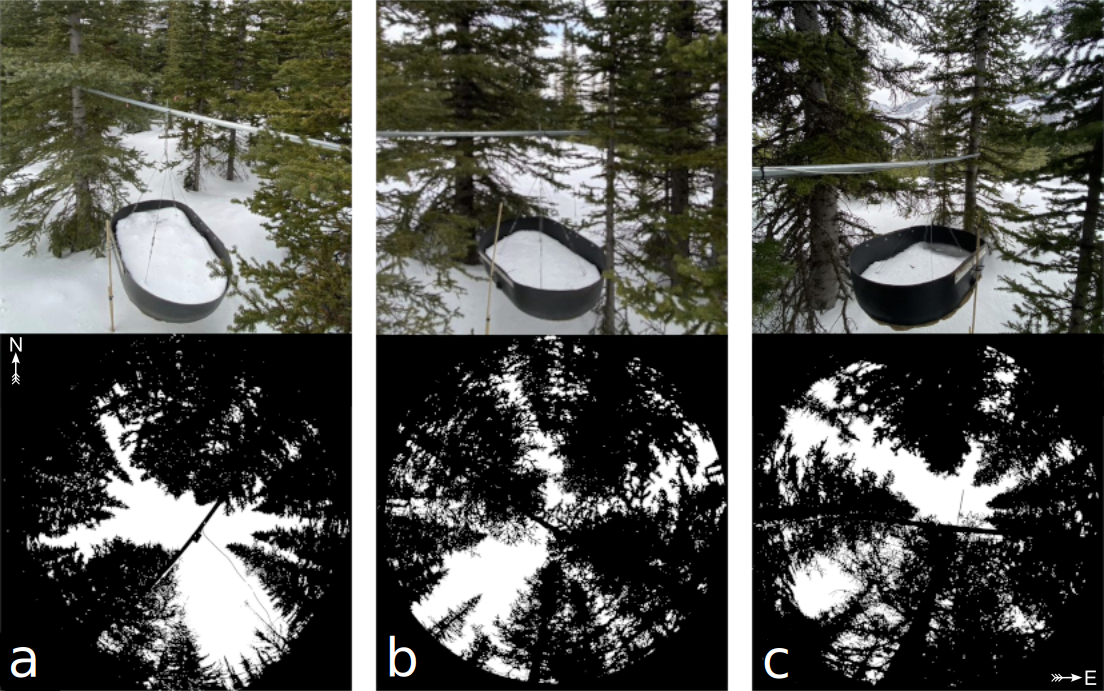
\includegraphics{figs/site-photos/scl_w_fisheye_textnew.png}

}

\caption{\label{fig-scl-imgs}Images of the three subcanopy lysimeter
instruments and surrounding canopy located in sparse (a), mixed (b), and
dense (c) canopy. The top row presents a side view of each instrument
and the bottom row shows hemispherical photographs. These hemispherical
images are oriented with north at the top and have been mirrored to
provide a view from above (e.g., east is on the right side of each
image). See Table~\ref{tbl-scl-lai-cc} for the corresponding canopy
density measurement.}

\end{figure}%

\subsection{UAV-Lidar data collection and
processing}\label{uav-lidar-data-collection-and-processing}

The UAV (FreeFly Alta X) payload included a REIGL miniVUX-2 airborne
laser scanner, an Applanix APX-20 inertial measurement unit (IMU) and
global navigation satellite system (GNSS). The UAV was flown 90 m above
the ground at a speed of 3 m s\textsuperscript{-1} following the path
shown in Figure~\ref{fig-site-map}. The methods outlined by Harder et
al. (2020) and Staines \& Pomeroy (2023) were incorporated to reconcile
survey lidar, IMU, and GNSS data. A systematic vertical bias of up to 6
cm between UAV-lidar flight lines was observed in the resulting point
clouds on March 13\textsuperscript{th} and 14\textsuperscript{th}, 2024
and was attributed to IMU position drift. After strip alignment, the
mean elevation bias in the point clouds compared to the GNSS data was
0.000 m and the RMS error declined from 0.055 m to 0.038 m on March
13\textsuperscript{th} and from 0.033 m to 0.029 m on March
14\textsuperscript{th}. The point cloud density ranged from
\textasciitilde1200 returns m\textsuperscript{2} in sparse forest to
\textasciitilde2200 returns m\textsuperscript{2} in open clearings.
Quality control, ground classification, calculation of surface elevation
change was conducted on the point cloud data and then converted to 0.05
m resolution rasters. Further quality control was conducted on the 0.05
m raster data to remove values that exceeded the .999th quantile and
then resampled to 0.25 m grid cell resolution by taking the median. A
detailed description of the UAV, payload, flight settings, and software
packages used is provided in the Supporting Information.

\subsection{Snow surveys}\label{snow-surveys}

\subsubsection{In-situ snow depth and
density}\label{in-situ-snow-depth-and-density}

Event-based snow surveys provided measurements of subcanopy throughfall
depth and density at 30 locations following the transects shown in
Figure~\ref{fig-site-map}. These measurements were used to upscale the
weighed tree from weight to weight per unit area, assess the accuracy of
lidar derived snow depth measurements, and provide a fresh snow density
for the calculation of SWE (mm) from the snow depth measurements.
Minimal ablation and redistribution of both the surface snowpack and/or
snow intercepted in the canopy was crucial to ensure the snow survey
measurements were attributed to throughfall. Therefore, only snowfall
events with minimal canopy snow ablation as determined through in-situ
observations, analysis of timelapse imagery, and mass change on the
weighed tree lysimeter were selected. A 1000 cm\textsuperscript{3} Perla
snow density wedge sampler (RIP Cutter,
https://snowmetrics.com/shop/rip-1-cutter-1000-cc/) was used to measure
the density of the fresh snow layer, \(\overline{\rho_{tf}}\) (kg
m\textsuperscript{-3}) from snow pits. Throughfall depth measurements,
\(\Delta HS\) were converted to SWE using the following equation:

\begin{equation}\phantomsection\label{eq-swe-tf}{
\Delta SWE_{tf} = \Delta HS \cdot \overline{\rho_{tf}}
}\end{equation}

If a pre-event crust layer was present, the depth of post event fresh
snow accumulation above the crust layer was interpreted as throughfall
over the event. In the absence of a defined crust layer, the difference
in pre- and post-event snow depth to ground was interpreted as event
throughfall. Interception efficiency, used in scaling the weighed tree,
was calculated using Equation~\ref{eq-ip2} and the \(\Delta SWE_{tf}\)
and cumulative snowfall measurements.

\subsubsection{UAV-Lidar snow depth}\label{uav-lidar-snow-depth}

Two uncrewed aerial vehicle (UAV) lidar surveys were conducted before
and after a 24-hour snowfall event that occurred between March
13--14\textsuperscript{th}, 2023 to facilitate the measurement of snow
accumulation and canopy density within the FT and PWL forest plots. This
period was selected based on two criteria: 1) it provided sufficient
cumulative snowfall to result in a low relative error in UAV-lidar
measured throughfall, and 2) minimal snow redistribution and ablation
was observed, as confirmed by the subcanopy lysimeters, weighed tree,
and time-lapse imagery. The change in surface elevation between the two
UAV-lidar point clouds was interpreted as the increase in snow
accumulation, \(\Delta HS\), over the snowfall event.
\(\Delta SWE_{tf}\) was calculated using Equation~\ref{eq-swe-tf}
together with in-situ measurements of \(\overline{\rho_{tf}}\). The
measurement error of the UAV-lidar derived \(\Delta HS\) was assessed
using the in-situ snow depth observations which is shown in the
Supporting Information. Spatially distributed measurements of
\(\frac{I}{P}\), were then determined using Equation~\ref{eq-ip2} with
\(\Delta SWE_{tf}\) as the throughfall component and cumulative snowfall
to the PWL clearing.

\subsection{UAV-Lidar canopy metrics}\label{uav-lidar-canopy-metrics}

The canopy of the study site was characterized from two UAV-lidar point
clouds (March 13\textsuperscript{th} and March 14\textsuperscript{th})
using the voxel ray sampling (VoxRS) methodology for lidar data
analysis, as developed by Staines \& Pomeroy (2023). This method was
chosen for its ability to provide canopy metrics that are less sensitive
to the inherent non-uniform nature of lidar sampling data resulting from
beam occlusion in vegetation. Using this method radiation transmittance,
\(\tau\) (-), was measured across the hemisphere at a 1° step, e.g.,
azimuth angles (0°, 1°, \ldots, 359°) and zenith angles (0°, 1°, \ldots,
90°) for each 0.25 m grid cell within the FT and PWL forest plots. The
fraction of snow-leaf contact area per unit area of ground proposed by
Hedstrom \& Pomeroy (1998), and hereafter called leaf contact area
(\(C_p\)), was then calculated as:

\begin{equation}\phantomsection\label{eq-lca}{
C_p(C_c, \theta_h) = 1-\tau
}\end{equation}

\begin{equation}\phantomsection\label{eq-tf-ode}{
C_p(C_c, \theta_h) = \begin{cases}
    1-\tau,& \text{if } \theta_h> 0°\\
    1-\tau \approx C_c ,              & \theta_h= 0°
\end{cases}
}\end{equation}

where \(C_p\) is a function of the canopy cover (\(C_c\)) and
hydrometeor trajectory angle (\(\theta_h\)). \(C_c\) is the fraction of
canopy area to total ground area when viewed from above, which differs
from canopy closure, an angular-derived metric usually measured from the
ground perspective.

To determine how \(C_p\) was associated with interception efficiency at
different azimuth and zenith angles over the March
13--14\textsuperscript{th} snowfall event, the entire hemisphere at each
grid location was considered. The relationship between interception
efficiency and \(C_p\) was found to be linear and thus the Pearson
Correlation Coefficient was used. The Pearson Correlation Coefficient
was computed between a single raster of interception efficiency and each
of the 32,760 rasters of \(C_p\) measured on March
13\textsuperscript{th}, representing locations across the hemisphere
(azimuth {[}0°, 1°, \ldots, 359°{]}, zenith angle {[}0°, 1°, \ldots,
90°{]}) at 0.25 m grid cells spanning the FT and PWL forest plots.

The pair of azimuth and zenith angles corresponding to the \(C_p\) that
had the highest correlation with interception efficiency was selected
for further analysis. This involved aggregating the interception
efficiency and selected \(C_p\) rasters from a 0.25 m resolution to 5 m,
followed by fitting an ordinary least squares regression between these
two variables. The regression was constrained to pass through the origin
based on the theoretical principle that the dependent variable must
equal zero when the independent variable is zero. To appropriately
account for this constraint, the \emph{R}\textsuperscript{2} values were
adjusted according to Equation 10 presented in Kozak \& Kozak (1995).
The relationship between leaf contact area and simulated trajectory
angle was investigated by fitting non-linear models using a non-linear
least squares regression. All statistical analyses were performed using
the R `stats' package (R Core Team, 2024).

\section{Results}\label{results}

\subsection{The influence of meteorology on snow
interception}\label{the-influence-of-meteorology-on-snow-interception}

Measurements of canopy snow load derived from the subcanopy lysimeters
and weighed tree increased linearly with cumulative event snowfall for
26 snowfall events, without evidence of reaching a maximum
(Figure~\ref{fig-scl-w-sf}). Over these events, air temperature ranged
from -24.5°C to 1°C, wind speeds at 4.3 m height ranged from calm to 4.6
m s\textsuperscript{-1} (Table~\ref{tbl-sf-event-met}), and wind
direction was predominately from the southwest during snowfall
(Figure~\ref{fig-wind-rose}). Missing canopy snow load measurements, as
shown in Figure~\ref{fig-scl-w-sf} for certain events, were caused by
wiring damage from animals and heavy snow loads. Some of the variability
in interception rates within and between different events may be
attributed to small amounts of canopy snow unloading and melt, which
could not be fully accounted for through the manual and automated
filtering mitigation strategies in both the subcanopy lysimeter and
weighed tree measurements.

\begin{figure}[H]

\centering{

\includegraphics{figs/automated_snowfall_event_periods/cuml_event_snowfall_canopy_storage_avg_of_scls_and_w_tree.png}

}

\caption{\label{fig-scl-w-sf}Plot showing the cumulative event snowfall
versus canopy snow load calculated using the mean of the three subcanopy
lysimeters (left) and weighed tree lysimeter (right) for each of the 26
snowfall events. Both datasets represent canopy snow load for a canopy
closure of 0.73 corresponding to the mean of the three subcanopy
lysimeter canopies.}

\end{figure}%

\pagebreak
\setstretch{1.0}

\begin{table}

\caption{\label{tbl-sf-event-met}Meteorology of the 26 snowfall events.
Air temperature and wind speed were measured at FT station. Interception
efficiency is estimated from cumulative snowfall measured at PWL station
and the average cumulative throughfall of all three subcanopy lysimeters
located within the FT forest plot.}

\centering{

\fontsize{12.0pt}{14.4pt}\selectfont
\begin{tabular*}{\linewidth}{@{\extracolsep{\fill}}>{\centering\arraybackslash}p{\dimexpr 67.50pt -2\tabcolsep-1.5\arrayrulewidth}>{\centering\arraybackslash}p{\dimexpr 37.50pt -2\tabcolsep-1.5\arrayrulewidth}>{\centering\arraybackslash}p{\dimexpr 37.50pt -2\tabcolsep-1.5\arrayrulewidth}>{\centering\arraybackslash}p{\dimexpr 37.50pt -2\tabcolsep-1.5\arrayrulewidth}>{\centering\arraybackslash}p{\dimexpr 37.50pt -2\tabcolsep-1.5\arrayrulewidth}>{\centering\arraybackslash}p{\dimexpr 37.50pt -2\tabcolsep-1.5\arrayrulewidth}>{\centering\arraybackslash}p{\dimexpr 37.50pt -2\tabcolsep-1.5\arrayrulewidth}>{\centering\arraybackslash}p{\dimexpr 37.50pt -2\tabcolsep-1.5\arrayrulewidth}>{\centering\arraybackslash}p{\dimexpr 37.50pt -2\tabcolsep-1.5\arrayrulewidth}>{\centering\arraybackslash}p{\dimexpr 37.50pt -2\tabcolsep-1.5\arrayrulewidth}>{\centering\arraybackslash}p{\dimexpr 60.00pt -2\tabcolsep-1.5\arrayrulewidth}}
\toprule
 & \multicolumn{3}{>{\centering\arraybackslash}m{\dimexpr 112.50pt -2\tabcolsep-1.5\arrayrulewidth}}{Air Temperature (°C)} & \multicolumn{3}{>{\centering\arraybackslash}m{\dimexpr 112.50pt -2\tabcolsep-1.5\arrayrulewidth}}{Wind Speed (m/s)} & \multicolumn{3}{>{\centering\arraybackslash}m{\dimexpr 112.50pt -2\tabcolsep-1.5\arrayrulewidth}}{Interception Efficiency (-)} & Snowfall (mm) \\ 
\cmidrule(lr){2-4} \cmidrule(lr){5-7} \cmidrule(lr){8-10} \cmidrule(lr){11-11}
Start Date & Min & Mean & Max & Min & Mean & Max & Min & Mean & Max & Total \\ 
\midrule\addlinespace[2.5pt]
2021-12-23 & -6.2 & -5.3 & -4.6 & 0.6 & 3.1 & 4.6 & 0.1 & 0.5 & 0.9 & 21.7 \\ 
2022-01-02 & -15.9 & -10.8 & -5.8 & 0.2 & 1.8 & 4.2 & 0.0 & 0.5 & 1.0 & 31.6 \\ 
2022-01-17 & -14.8 & -7.8 & -0.8 & 0.2 & 1.1 & 1.8 & 0.0 & 0.6 & 1.0 & 12.9 \\ 
2022-01-31 & -24.5 & -12.1 & -6.4 & 0.1 & 1.0 & 1.7 & 0.2 & 0.7 & 1.0 & 9.1 \\ 
2022-02-14 & -9.9 & -9.0 & -8.5 & 0.4 & 0.8 & 1.2 & 0.2 & 0.5 & 0.8 & 1.7 \\ 
2022-02-19 & -4.7 & -3.2 & -2.5 & 1.3 & 2.3 & 3.6 & 0.3 & 0.6 & 0.9 & 11.1 \\ 
2022-03-01 & -8.3 & -5.4 & -1.0 & 0.1 & 1.0 & 3.1 & 0.4 & 0.8 & 1.0 & 9.9 \\ 
2022-03-07 & -12.5 & -8.6 & -4.4 & 0.3 & 0.8 & 1.7 & 0.3 & 0.7 & 1.0 & 9.5 \\ 
2022-03-14 & -2.7 & -2.1 & -0.8 & 1.0 & 1.6 & 2.9 & 0.2 & 0.6 & 0.9 & 8.4 \\ 
2022-03-19 & -3.1 & -2.8 & -2.5 & 0.0 & 0.7 & 1.3 & 0.3 & 0.5 & 0.6 & 6.6 \\ 
2022-03-23 & -7.9 & -5.3 & -0.9 & 0.8 & 1.2 & 1.8 & 0.4 & 0.6 & 0.9 & 1.6 \\ 
2022-04-04 & -3.5 & -2.9 & -2.1 & 0.6 & 1.0 & 1.9 & 0.0 & 0.4 & 0.6 & 3.4 \\ 
2022-04-18 & -5.2 & -4.0 & -2.7 & 0.4 & 1.1 & 1.9 & 0.1 & 0.5 & 0.9 & 7.4 \\ 
2022-04-22 & -2.8 & -1.8 & -0.5 & 0.4 & 0.8 & 1.2 & 0.1 & 0.5 & 1.0 & 9.8 \\ 
2022-05-09 & -4.9 & -4.3 & -3.2 & 0.1 & 0.4 & 0.9 & 0.2 & 0.5 & 0.9 & 8.1 \\ 
2022-05-19 & -4.9 & -2.1 & 0.3 & 0.1 & 0.4 & 0.9 & 0.2 & 0.6 & 0.9 & 7.1 \\ 
2022-06-13 & -1.1 & -0.3 & 0.6 & 0.1 & 0.1 & 0.4 & 0.0 & 0.5 & 0.9 & 45.4 \\ 
2022-12-27 & -3.0 & -2.7 & -1.9 & 0.6 & 1.1 & 1.8 & 0.2 & 0.5 & 0.9 & 4.5 \\ 
2023-01-27 & -11.5 & -7.3 & -4.5 & 0.6 & 0.9 & 1.2 & 0.1 & 0.5 & 0.8 & 10.4 \\ 
2023-02-19 & -14.3 & -9.5 & -6.3 & 0.2 & 0.8 & 1.4 & 0.2 & 0.7 & 1.0 & 18.1 \\ 
2023-02-26 & -9.2 & -8.4 & -6.6 & 0.2 & 1.0 & 2.1 & 0.3 & 0.5 & 1.0 & 5.4 \\ 
2023-03-13 & -8.9 & -3.6 & -0.1 & 0.3 & 1.3 & 2.2 & 0.0 & 0.5 & 1.0 & 27.4 \\ 
2023-03-24 & -7.9 & -5.7 & -3.5 & 0.1 & 0.5 & 1.2 & 0.1 & 0.4 & 0.7 & 23.8 \\ 
2023-04-01 & -8.9 & -7.7 & -4.7 & 0.1 & 0.6 & 1.4 & 0.4 & 0.6 & 0.8 & 11.4 \\ 
2023-04-10 & -1.1 & -0.5 & 0.3 & 0.1 & 0.3 & 1.0 & 0.2 & 0.4 & 0.6 & 18.0 \\ 
2023-05-08 & 0.2 & 0.6 & 1.0 & 0.4 & 0.6 & 0.8 & 0.6 & 0.6 & 0.7 & 3.5 \\ 
\bottomrule
\end{tabular*}

}

\end{table}%

\setstretch{1.5}

\begin{figure}[H]

\centering{

\includegraphics[width=0.6\textwidth,height=\textheight]{figs/automated_snowfall_event_periods/ft_wind_rose_allevents_snowing_custom_dimensions.png}

}

\caption{\label{fig-wind-rose}Wind rose showing the frequency of wind
speed and direction over the 26 snowfall periods for the ultrasonic
anemometer 4.3 m above ground at FT station.}

\end{figure}%

Linear regression analysis revealed no relationship between hourly
interception efficiency (from the subcanopy lysimeters) and air
temperature, wind speed or canopy snow load, either due to
non-significant relationships (\emph{p} \textless{} 0.05) and/or weak
predictive power (\emph{R}\textsuperscript{2} \textless{} 0.05)
(Table~\ref{tbl-lysimeter-hourly-stats}). The Wilcoxon test indicated
that the difference in hourly interception efficiencies for air
temperatures above and below -5°C was not significant (\emph{p}
\textgreater{} 0.05, Table~\ref{tbl-scl-hrly-stats}). Additionally, the
interception efficiency across differing bins of air temperature did not
show any systematic pattern (Figure~\ref{fig-scl-ip-bins}). Although
Figure~\ref{fig-scl-ip-bins} indicates potentially higher interception
efficiency in sparse and mixed canopies at air temperatures below -10°C,
these measurements have substantial uncertainty due to heightened
instrument error associated with the small accumulations of snowfall and
throughfall within these temperature ranges.

When examining wind speed effects, hourly interception efficiencies were
found to be significantly higher (\emph{p} \textless{} 0.05,
Table~\ref{tbl-scl-hrly-stats}) during periods when wind speeds exceeded
1 m s\textsuperscript{-1} compared to calmer conditions in the sparse
and closed canopies using the Wilcoxon test. The binned data also show
an increase in interception efficiency with increasing wind speed for
these two canopy types (Figure~\ref{fig-scl-ip-bins}). In contrast, the
mixed canopy, which had a canopy opening towards the prevailing wind
direction (Figure~\ref{fig-scl-imgs}), exhibited no significant
difference (\emph{p} \textgreater{} 0.05,
Table~\ref{tbl-scl-hrly-stats}). Binned measurements of interception
efficiencies corresponding to wind speed bins above 2 m
s\textsuperscript{-1} (Figure~\ref{fig-scl-ip-bins}) contained
considerable uncertainty resulting from lower snowfall and throughfall
accumulation, reducing confidence in these particular findings across
all three canopy environments.

Significantly higher hourly interception efficiencies (\emph{p}
\textless{} 0.05, Table~\ref{tbl-scl-hrly-stats}) were found for initial
canopy snow loads below 10 mm compared to heavier snow loads across all
three canopy types using the Wilcoxon test. Additionally, the sparse and
mixed canopies exhibited significantly lower interception efficiencies
(\emph{p} \textless{} 0.05) for snow loads below 5 mm compared to those
between 5--10 mm. The closed canopy displayed a similar initial increase
for the binned data visible in Figure~\ref{fig-scl-ip-bins}, but this
was not statistically significant for the hourly data (\emph{p}
\textgreater{} 0.05, Table~\ref{tbl-scl-hrly-stats}). For the sparse and
closed canopies, a slight increase in binned interception efficiency was
observed as snow load increased up to 10 mm, followed by a decline when
snow loads exceeded 10 mm (Figure~\ref{fig-scl-ip-bins}). For snow loads
exceeding 15 mm, interception efficiency decreased in the sparse and
closed canopies, while the mixed canopy showed an increase; however,
these measurements carried high uncertainties due to lower accumulated
snowfall and throughfall in these higher snow load bins. The differences
between the relationships observed in the hourly-interval and binned
interception efficiency measurements can be attributed to two factors:
greater instrument uncertainty in the hourly measurements and the
potential for the dependent and independent variables to be
non-stationary over the hourly interval.

\begin{longtable}[]{@{}
  >{\raggedright\arraybackslash}p{(\columnwidth - 10\tabcolsep) * \real{0.3500}}
  >{\raggedright\arraybackslash}p{(\columnwidth - 10\tabcolsep) * \real{0.1500}}
  >{\raggedleft\arraybackslash}p{(\columnwidth - 10\tabcolsep) * \real{0.1000}}
  >{\raggedleft\arraybackslash}p{(\columnwidth - 10\tabcolsep) * \real{0.1700}}
  >{\raggedleft\arraybackslash}p{(\columnwidth - 10\tabcolsep) * \real{0.1300}}
  >{\raggedleft\arraybackslash}p{(\columnwidth - 10\tabcolsep) * \real{0.1000}}@{}}

\caption{\label{tbl-lysimeter-hourly-stats}Statistics corresponding to
the ordinary least squares linear regression test between hourly
interval measurements of independent variables: mean air temperature,
mean wind speed, and initial canopy snow load and the dependent variable
mean interception efficiency. The test was run separately for three
levels of canopy coverage (\(C_c\)) corresponding to each subcanopy
lysimeter (SCL).}

\tabularnewline

\toprule\noalign{}
\begin{minipage}[b]{\linewidth}\raggedright
Dependent Variable
\end{minipage} & \begin{minipage}[b]{\linewidth}\raggedright
SCL Name
\end{minipage} & \begin{minipage}[b]{\linewidth}\raggedleft
\(C_c\)
\end{minipage} & \begin{minipage}[b]{\linewidth}\raggedleft
Adjusted \(R^2\)
\end{minipage} & \begin{minipage}[b]{\linewidth}\raggedleft
\(p\)-value
\end{minipage} & \begin{minipage}[b]{\linewidth}\raggedleft
\(n\)
\end{minipage} \\
\midrule\noalign{}
\endhead
\bottomrule\noalign{}
\endlastfoot
Air Temperature (°C) & closed & 0.79 & 0.002 & 0.239 & 191 \\
Air Temperature (°C) & mixed & 0.75 & 0.024 & 0.005 & 298 \\
Air Temperature (°C) & sparse & 0.64 & 0.003 & 0.208 & 190 \\
Initial Canopy Snow Load (mm) & closed & 0.79 & 0.029 & 0.011 & 188 \\
Initial Canopy Snow Load (mm) & mixed & 0.75 & 0.010 & 0.049 & 294 \\
Initial Canopy Snow Load (mm) & sparse & 0.64 & 0.031 & 0.009 & 187 \\
Wind Speed (m/s) & closed & 0.79 & 0.025 & 0.017 & 191 \\
Wind Speed (m/s) & mixed & 0.75 & 0.034 & 0.001 & 298 \\
Wind Speed (m/s) & sparse & 0.64 & 0.046 & 0.002 & 190 \\

\end{longtable}

\begin{figure}[H]

\centering{

\includegraphics{figs/automated_snowfall_event_periods/troughs_met_vs_IP_accumulated_bin.png}

}

\caption{\label{fig-scl-ip-bins}Scatter plots showing the interception
efficiency calculated from accumulated snowfall (Pluvio) and throughfall
(subcanopy lysimeter) measurements for bins of air temperature, wind
speed, and initial canopy snow load (the snow load observed by the
weighed tree at the beginning of the timestep) over the 26 snowfall
events. The error bars represent the estimated combined instrument error
of the snowfall gauge and subcanopy lysimeters.}

\end{figure}%

\begin{longtable}[]{@{}
  >{\raggedright\arraybackslash}p{(\columnwidth - 10\tabcolsep) * \real{0.1200}}
  >{\raggedright\arraybackslash}p{(\columnwidth - 10\tabcolsep) * \real{0.3000}}
  >{\raggedright\arraybackslash}p{(\columnwidth - 10\tabcolsep) * \real{0.1200}}
  >{\raggedright\arraybackslash}p{(\columnwidth - 10\tabcolsep) * \real{0.1800}}
  >{\raggedright\arraybackslash}p{(\columnwidth - 10\tabcolsep) * \real{0.1500}}
  >{\raggedright\arraybackslash}p{(\columnwidth - 10\tabcolsep) * \real{0.1300}}@{}}

\caption{\label{tbl-scl-hrly-stats}Results of the Wilcoxon signed-rank
tests comparing the distributions of hourly interception efficiency (IP)
measured by the subcanopy lysimeters for differing groups of air
temperatures (Ta), wind speeds (u), and initial canopy snow loads (L).
The table reports the canopy corresponding to the subcanopy lysimeter
(Canopy), null hypothesis (\(H_0\)), \(p\)-value, and sample size
(\(n\)) and median IP for the `low' group (e.g., Ta \textless{} -5°C)
and `high' group (e.g., Ta ≥ -5°C).}

\tabularnewline

\toprule\noalign{}
\begin{minipage}[b]{\linewidth}\raggedright
Canopy
\end{minipage} & \begin{minipage}[b]{\linewidth}\raggedright
Null Hypothesis (\(H_0\))
\end{minipage} & \begin{minipage}[b]{\linewidth}\raggedright
\(p\)-value
\end{minipage} & \begin{minipage}[b]{\linewidth}\raggedright
\(n\) (low / high)
\end{minipage} & \begin{minipage}[b]{\linewidth}\raggedright
median I/P (low / high)
\end{minipage} & \begin{minipage}[b]{\linewidth}\raggedright
Reject \(H_0\)
\end{minipage} \\
\midrule\noalign{}
\endhead
\bottomrule\noalign{}
\endlastfoot
closed & Median IP (Ta \textless{} -5°C) ≥ Median IP (Ta ≥ -5°C) & 0.282
& 76 / 115 & 0.56 / 0.62 & no \\
mixed & Median IP (Ta \textless{} -5°C) ≥ Median IP (Ta ≥ -5°C) & 0.990
& 165 / 133 & 0.57 / 0.53 & no \\
sparse & Median IP (Ta \textless{} -5°C) ≥ Median IP (Ta ≥ -5°C) & 0.864
& 72 / 118 & 0.54 / 0.5 & no \\
closed & Median IP (u \textless{} 1 m/s) ≥ Median IP (u ≥ 1 m/s) & 0.004
& 116 / 75 & 0.53 / 0.65 & yes \\
mixed & Median IP (u \textless{} 1 m/s) ≥ Median IP (u ≥ 1 m/s) & 1.000
& 165 / 133 & 0.6 / 0.5 & no \\
sparse & Median IP (u \textless{} 1 m/s) ≥ Median IP (u ≥ 1 m/s) &
\textless{} 0.001 & 110 / 80 & 0.43 / 0.59 & yes \\
closed & Median IP (L \textless{} 10 mm) ≤ Median IP (L ≥ 10 mm) & 0.048
& 129 / 59 & 0.62 / 0.57 & yes \\
mixed & Median IP (L \textless{} 10 mm) ≤ Median IP (L ≥ 10 mm) &
\textless{} 0.001 & 218 / 76 & 0.57 / 0.49 & yes \\
sparse & Median IP (L \textless{} 10 mm) ≤ Median IP (L ≥ 10 mm) &
\textless{} 0.001 & 157 / 30 & 0.53 / 0.34 & yes \\
closed & Median IP (L \textless{} 5 mm) ≥ Median IP (5 mm ≤ L
\textless{} 10 mm) & 0.333 & 62 / 67 & 0.62 / 0.62 & no \\
mixed & Median IP (L \textless{} 5 mm) ≥ Median IP (5 mm ≤ L \textless{}
10 mm) & 0.019 & 117 / 101 & 0.57 / 0.61 & yes \\
sparse & Median IP (L \textless{} 5 mm) ≥ Median IP (5 mm ≤ L
\textless{} 10 mm) & 0.043 & 90 / 67 & 0.49 / 0.6 & yes \\

\end{longtable}

\subsection{The influence of canopy density on snow
interception}\label{the-influence-of-canopy-density-on-snow-interception}

UAV-lidar measurements of throughfall and canopy density provide
insights on how the forest canopy influenced subcanopy snow accumulation
during a wind-driven snowfall event between March
13--14\textsuperscript{th}. This event totaled 28.7 mm of snowfall at
PWL station and was characterized by a transition from low rates of
snowfall and air temperatures near 0°C to higher rates of snowfall by
late afternoon on March 13\textsuperscript{th} coinciding with air
temperatures around -2.5 °C. An average wind speed of 1.3 m
s\textsuperscript{-1} and direction of 188° was observed 4.3 m above the
ground at FT Station. The mean observed hydrometeor terminal fall
velocity observed over the event was 0.9 m s\textsuperscript{-1}.

The throughfall depth measured by UAV-lidar aligned with the in-situ
manual measurements resulting in a mean bias of -0.001 m and RMSE of
0.024 m. More details on the accuracy of UAV-lidar snow depth
measurements are provided in the Supporting Information section.
Figure~\ref{fig-lidar-tf-ip} shows the spatial distribution of
throughfall and interception efficiency at the PWL and FT forest plots.
Reduced throughfall and greater interception efficiency was observed on
the north (lee) side of individual trees, which may be due to
non-vertical hydrometeor trajectories caused by the steady southerly
winds observed over this event. Transparent areas within the forest
plots in Figure~\ref{fig-lidar-tf-ip} represent grid cells that did not
have any lidar ground returns (e.g., under dense canopy proximal to tree
trunks) or were masked due to disturbance (e.g., walking paths in
clearings). Visual observations on March 13\textsuperscript{th} and
14\textsuperscript{th} confirmed non-vertical hydrometeor trajectories
and increased canopy snow loads were observed on the windward side of
individual trees. This effect is more apparent in the PWL forest plot
than the FT forest plot and may be attributed to the taller trees and
higher canopy cover of the PWL forest plot compared to the FT forest
plot (Figure~\ref{fig-lidar-tf-ip}).

\begin{figure}[H]

\centering{

\includegraphics{figs/external_figures/facet_ft_pwl_23_072_23_073_v2.0.0_saswe_and_ip_normalised_resample_0.25.png}

}

\caption{\label{fig-lidar-tf-ip}UAV-lidar measurements of the change in
snow water equivalent, SWE (mm) and interception efficiency, I/P (-),
over the March 13--14\textsuperscript{th} 24-hour snowfall event for the
FT and PWL forest plots at a 0.25 m resolution. See the location of the
two forest plots in Figure~\ref{fig-site-map}.}

\end{figure}%

The VoxRS measurements of \(C_p\) on March 13\textsuperscript{th} were
selected for analysis and represent the canopy of both forest plots
without snow. Little difference in \(C_p\) was observed between the
March 13\textsuperscript{th} and March 14\textsuperscript{th}
measurements. A strong linear correlation between \(C_p\) measured on
March 13\textsuperscript{th} and interception efficiency was observed
towards the southern portion of the hemisphere, aligning with the
average event wind direction (Figure~\ref{fig-hemi-ip-cc}). For the PWL
forest plot, the upper 97.5\textsuperscript{th} percentile of the
Pearson Correlation Coefficient (\(\rho_p\)) values were found between
azimuth angles of 167°--217°. Similarly, for the FT forest plot, the
upper 97.5\textsuperscript{th} percentile of \(\rho_p\) was found
between azimuth angles of 171°--223°. The zenith angle found to have the
highest correlation over this azimuth range was 22° (\(\rho_p\) = 0.7)
and 21° (\(\rho_p\) = 0.83) for PWL and FT respectively. The high
correlation coefficients found for non-vertical zenith angles for both
PWL and FT are hypothesized to result from non-vertical hydrometeor
trajectories.

\begin{figure}[H]

\centering{

\includegraphics{figs/external_figures/full_hemi_rho_p_cor_lca_ip_23_072_vox_len_0.25m_sa_gridgen_v2.0.0_sa_ft_pwl_.png}

}

\caption{\label{fig-hemi-ip-cc}The Pearson Correlation Coefficient
between rasters (0.25 m resolution) of interception efficiency and leaf
contact area (measured on March 13th) for each grid cell across the
study site for each azimuth angles (0°, 1°, \ldots, 359°) and zenith
angles (0°, 1°, \ldots, 90°) for the FT (left) and PWL (right) forest
plots.}

\end{figure}%

The spatial distribution of \(C_p\) measurements, selected based on the
vector corresponding to the azimuth and zenith angles observed to have
the highest correlation with interception efficiency in
Figure~\ref{fig-hemi-ip-cc}, is shown in Figure~\ref{fig-lidar-cc-cp}.
These \(C_p\) measurements generally align with the spatial distribution
of interception efficiency and throughfall
(Figure~\ref{fig-lidar-tf-ip}).

\begin{figure}[H]

\centering{

\includegraphics{figs/external_figures/facet_ft_pwl_23_072_vox_len_0.25m_sa_gridgen_v2.0.0_sa__leaf_contact_area_event_traj_25cm.png}

}

\caption{\label{fig-lidar-cc-cp}UAV-lidar VoxRS measurements of leaf
contact area measured on March 13\textsuperscript{th} for the PWL and FT
forest plots for zenith angles (PWL = 22°, FT = 21°) and azimuth angles
(PWL = 167°, 178°, \ldots{} 217°; FT = 171°, 172°, \ldots{} 223°).}

\end{figure}%

The correlation between interception efficiency
(Figure~\ref{fig-lidar-tf-ip}) and \(C_p\)
(Figure~\ref{fig-lidar-cc-cp}), resampled to a 5 m grid resolution, was
higher compared to the association with leaf contact angle measured at a
zenith angle of 0° (Figure~\ref{fig-lca-vs-ip}). The stronger
association for the vector-based calculation is hypothesized to stem
from a more accurate representation of the snowfall contact area and
suggests that adjusted \(C_p\) is a useful predictor of interception
efficiency before ablation. An ordinary least squares linear regression
forced through the origin was fit to the observed data points using the
following equation:

\begin{equation}\phantomsection\label{eq-lca-ip}{
  \frac{I}{P} = C_p(C_c, \theta_h) \cdot \alpha
}\end{equation}

where \(\alpha\) is an efficiency constant which determines the fraction
of snowflakes that contact the \(C_p\) elements and are stored in the
canopy (i.e., intercepted) before canopy snow unloading or ablation
processes begin.

\begin{figure}[H]

\centering{

\includegraphics{figs/external_figures/pwl_ft_lca_vs_ip_phi_nadir_adjusted_resample_w_mods_5m.png}

}

\caption{\label{fig-lca-vs-ip}Scatter plots showing the relationship
between leaf contact area and interception efficiency rasters resampled
to a 5 m grid cell resolution. The left plot (nadir) shows canopy
coverage and the right plot (Vector Based) shows the leaf contact area
averaged over rasters with zenith angles (PWL = 22°, FT = 21°) and
azimuth angles (PWL = 167°, 178°, \ldots{} 217°; FT = 171°, 172°,
\ldots{} 223°). The solid lines (Model fit) show an ordinary least
squares linear regression forced through the origin and fitted to the
PWL (red) and FT (black) data and the light grey dotted line shows a 1:1
line. The \emph{R}\textsuperscript{2} values for the four different
models are shown in the upper left of each panel calculated following
the methods outlined in Kozak \& Kozak (1995).}

\end{figure}%

For the vector-based model, the relationship between interception
efficiency and \(C_p\) resulted in \emph{R}\textsuperscript{2} values of
0.45 and 0.8 for PWL and FT respectively. Model error statistics show
the vector-based model provided a better prediction of interception
efficiency compared to the nadir canopy coverage measurements
(Table~\ref{tbl-ip-mod-err}). The increase in interception efficiency
with \(C_p\) follows a reduced slope compared to the nadir models with
\(\alpha\) values of 0.72 and 0.69 for the PWL and FT vector-based
models respectively. The reduced slope for the vector-based models may
be due to snowflakes that weaved through and/or bounced off branch
elements in addition to UAV-lidar throughfall measurement uncertainty
which may have been slightly affected by unloading and redistribution.
These processes would have reduced the fraction of snowfall that was
stored in the canopy. Some of the scatter observed in the nadir model
shown in Figure~\ref{fig-lca-vs-ip} may be explained by grid cells
within canopy gaps which observed a greater interception efficiency
compared to the corresponding canopy cover. Conversely, grid cells where
interception efficiency is less than the canopy cover, may be affected
by non-vertical trajectory hydrometeors making their way underneath the
canopy as observed by the reduced interception efficiency on the
windward edges of individual trees in Figure~\ref{fig-lidar-tf-ip}.

\pagebreak

\begin{longtable}[]{@{}
  >{\raggedright\arraybackslash}p{(\columnwidth - 12\tabcolsep) * \real{0.1000}}
  >{\raggedright\arraybackslash}p{(\columnwidth - 12\tabcolsep) * \real{0.2500}}
  >{\raggedleft\arraybackslash}p{(\columnwidth - 12\tabcolsep) * \real{0.1500}}
  >{\raggedleft\arraybackslash}p{(\columnwidth - 12\tabcolsep) * \real{0.1500}}
  >{\raggedleft\arraybackslash}p{(\columnwidth - 12\tabcolsep) * \real{0.1000}}
  >{\raggedleft\arraybackslash}p{(\columnwidth - 12\tabcolsep) * \real{0.1200}}
  >{\raggedleft\arraybackslash}p{(\columnwidth - 12\tabcolsep) * \real{0.1300}}@{}}

\caption{\label{tbl-ip-mod-err}Summary of error statistics for the
linear regression models relating leaf contact area to interception
efficiency, presented in Figure~\ref{fig-lca-vs-ip}. The Mean bias is
the difference in the model and observed values, MAE is the mean of the
absolute error, RMS Error is the root mean squared error,
\emph{R}\textsuperscript{2} is the coefficient of determination adjusted
using Equation 10 in Kozak \& Kozak (1995).}

\tabularnewline

\toprule\noalign{}
\begin{minipage}[b]{\linewidth}\raggedright
Plot Name
\end{minipage} & \begin{minipage}[b]{\linewidth}\raggedright
Canopy Calculation
\end{minipage} & \begin{minipage}[b]{\linewidth}\raggedleft
Model Slope (-)
\end{minipage} & \begin{minipage}[b]{\linewidth}\raggedleft
Mean Bias (-)
\end{minipage} & \begin{minipage}[b]{\linewidth}\raggedleft
MAE (-)
\end{minipage} & \begin{minipage}[b]{\linewidth}\raggedleft
RMS Error (-)
\end{minipage} & \begin{minipage}[b]{\linewidth}\raggedleft
\(R^2\)
\end{minipage} \\
\midrule\noalign{}
\endhead
\bottomrule\noalign{}
\endlastfoot
FT & Nadir & 1.01 & 0.024 & 0.072 & 0.101 & 0.49 \\
FT & Vector Based & 0.69 & 0.003 & 0.047 & 0.063 & 0.80 \\
PWL & Nadir & 0.96 & 0.049 & 0.115 & 0.148 & -0.31 \\
PWL & Vector Based & 0.72 & 0.020 & 0.079 & 0.096 & 0.45 \\

\end{longtable}

\subsection{The combined influence of trajectory angle and canopy
density on snow
interception}\label{the-combined-influence-of-trajectory-angle-and-canopy-density-on-snow-interception}

VoxRS measurements of \(C_p\) prior to snowfall on March
13\textsuperscript{th}, increased substantially with simulated
hydrometeor trajectory angle and corresponding simulated wind speed
(Figure~\ref{fig-lca-ht-ws}). The standard deviation in VoxRS measured
\(C_p\), illustrated by the shaded area in Figure~\ref{fig-lca-ht-ws},
exhibits the broad range in values for individual grid cells across each
forest plot. Despite this large scatter, a systematic increase in the
mean \(C_p\) across both forest plots results from a rise in the number
of canopy elements for more horizontal angles, when averaged across each
forest plot, over all azimuth angles (see top left panel
Figure~\ref{fig-lca-ht-ws}). This results in a large rise in \(C_p\)
over relatively common wind speeds. For example, with a wind speed of 1
m s\textsuperscript{-1} and estimated trajectory angle of 48°, \(C_p\)
would increase by 0.31 and 0.28 for the PWL and FT forest plots
respectively (Figure~\ref{fig-lca-ht-ws}). The increase in \(C_p\) from
nadir measured canopy coverage with increasing trajectory angle exhibits
a similar relationship for both forest plots FT and PWL until trajectory
angles reach approximately 60° (see bottom row of
Figure~\ref{fig-lca-ht-ws}). Beyond 60°, the PWL rate of increase slows
as the \(C_p\) approaches 1.0, while the FT plot, which has lower canopy
coverage, continues to rise until around 75° as a \(C_p\) of 1.0 is
approached. \(C_p\) was also quantified across trajectory angles for
both PWL and FT on March 14\textsuperscript{th}, post snowfall, and
showed a negligible increase in \(C_p\) compared to \(C_p\) measured on
March 13\textsuperscript{th} without snow in the canopy.

\begin{figure}[H]

\centering{

\includegraphics{figs/external_figures/WITH_TREEWELLS_traj_angle_and_wind_single_zenith_1_thetaby_1_traj_angle_wind_speed_vs_cowplot_lca_and_inc_w_mods_mean_sd_23_072.png}

}

\caption{\label{fig-lca-ht-ws}Plots showing the relationship between
hydrometeor trajectory angle (left column) and wind speed (right column)
with mean plot-wide snow-leaf contact area, \(C_p\) (top row) and the
increase in mean plot-wide \(C_p\), i.e., \(C_p - C_c\) (bottom row).
The simulated hydrometeor trajectory angle is measured as degrees from
zenith. Simulated wind speed was calculated as a function of hydrometeor
trajectory angle by rearranging Equation~\ref{eq-ta} and an observed
event hydrometeor fall velocity of 0.9 m s\textsuperscript{-1}. The
solid lines (VoxRS) represent the mean \(C_p\) (top row) or increase in
mean \(C_p\) (bottom row) for a single zenith angle observed from VoxRS
across all grid cells for each forest plot and across all azimuth
angles. The shaded area represents one standard deviation above and
below the observed VoxRS mean. The dashed lines (Fitted) represent
predictions from Equation~\ref{eq-lca-ac} (top row) and
Equation~\ref{eq-lca-inc} (bottom row). The dotted lines (HP98)
represent the predictions from Equation 10 in Hedstrom \& Pomeroy
(1998). A forested downwind distance of 100 m was assumed for the HP98
calculation.}

\end{figure}%

A function is proposed here to calculate plot-scale leaf contact area,
\(C_p\) (-):

\begin{equation}\phantomsection\label{eq-lca-ac}{
C_p = C_c + C_{inc}(\theta_h, C_c)
}\end{equation}

where \(C_{inc}\) represents the increase in leaf contact area from
nadir measured canopy coverage (\(C_c\)), and is a function of
\(\theta_h\) and \(C_c\). To estimate \(C_{inc}\) in the absence of
detailed canopy measurements, the following function is proposed:

\begin{equation}\phantomsection\label{eq-lca-inc}{
C_{inc} = (1-C_c)\cdot f(\theta_h)
}\end{equation}

where \(1-C_C\) quantifies the available void space within the canopy
and \(f(\theta_h)\) represents the fraction of that space contributing
to increased leaf contact area. Here, \(f(\theta_h)\) is approximated
as:

\begin{equation}\phantomsection\label{eq-f-theta}{
f(\theta_h) = b \cdot\text{sin}(\theta_h)^2
}\end{equation}

where \(b\) is a fitting coefficient, estimated to be
\textasciitilde0.91 through a non-linear least squares regression fit to
the VoxRS measurements at both FT and PWL. The term
\(\text{sin}(\theta_h)^2\) reflects the relative increase in snow-leaf
contact area, which in turn leads to a proportional decrease in the
canopy void space (\(1-C_c\)). Thus, for \(\theta_h\) of 0°, \(C_p\) is
equal to the canopy cover. In contrast, for \(\theta_h\) close to 90°,
\(C_p\) approaches a value of 1.0. The assumptions of
Equation~\ref{eq-f-theta} include that \(C_c\) represents a measurement
of continuous canopy cover without large open areas many times greater
than the mean canopy height and that snowfall trajectories are linear.

Simulated \(C_p\) using Equation~\ref{eq-lca-ac} is shown in the dashed
lines in the top row of Figure~\ref{fig-lca-ht-ws} and follows the
VoxRS-measured mean \(C_p\) closely. Model error statistics demonstrate
that Equation~\ref{eq-lca-inc} performed well, with a mean bias and RMSE
of -0.05 (-) and 0.05 (-) for PWL, and 0.03 (-) and 0.05 (-) for FT
respectively (Table~\ref{tbl-lca-mod-err}). In contrast, the Hedstrom \&
Pomeroy (1998) method produced significantly less accurate estimates of
\(C_p\), with a mean bias and RMSE of -0.2 (-) and 0.23 (-) for PWL, and
-0.26 (-) and 0.32 (-) for FT respectively
(Table~\ref{tbl-lca-mod-err}).

\begin{longtable}[]{@{}
  >{\raggedright\arraybackslash}p{(\columnwidth - 10\tabcolsep) * \real{0.1500}}
  >{\raggedright\arraybackslash}p{(\columnwidth - 10\tabcolsep) * \real{0.1700}}
  >{\raggedleft\arraybackslash}p{(\columnwidth - 10\tabcolsep) * \real{0.1700}}
  >{\raggedleft\arraybackslash}p{(\columnwidth - 10\tabcolsep) * \real{0.1500}}
  >{\raggedleft\arraybackslash}p{(\columnwidth - 10\tabcolsep) * \real{0.2000}}
  >{\raggedleft\arraybackslash}p{(\columnwidth - 10\tabcolsep) * \real{0.1700}}@{}}

\caption{\label{tbl-lca-mod-err}Model error statistics calculated for
the prediction of leaf contact area from trajectory angle using
Equation~\ref{eq-lca-inc} and Equation 10 from Hedstrom \& Pomeroy
(1998) (HP98) for the PWL and FT forest plots. Mean bias is the
difference in the model and observed values, MAE is the mean of the
absolute error, RMS Error is the root mean squared error and
\emph{R}\textsuperscript{2} is the coefficient of determination. The
units for all metrics are dimensionless. A forested downwind distance of
100 m was used for the HP98 calculation.}

\tabularnewline

\toprule\noalign{}
\begin{minipage}[b]{\linewidth}\raggedright
Model
\end{minipage} & \begin{minipage}[b]{\linewidth}\raggedright
Plot Name
\end{minipage} & \begin{minipage}[b]{\linewidth}\raggedleft
Mean Bias (-)
\end{minipage} & \begin{minipage}[b]{\linewidth}\raggedleft
MAE (-)
\end{minipage} & \begin{minipage}[b]{\linewidth}\raggedleft
RMS Error (-)
\end{minipage} & \begin{minipage}[b]{\linewidth}\raggedleft
\(R^2\)
\end{minipage} \\
\midrule\noalign{}
\endhead
\bottomrule\noalign{}
\endlastfoot
HP98 & FT & -0.26 & 0.26 & 0.32 & -0.97 \\
HP98 & PWL & -0.20 & 0.20 & 0.23 & -0.96 \\
Eq. 10 & FT & 0.03 & 0.04 & 0.05 & 0.95 \\
Eq. 10 & PWL & -0.05 & 0.05 & 0.05 & 0.90 \\

\end{longtable}

\subsection{Throughfall model
performance}\label{throughfall-model-performance}

The performance of the interception efficiency
(Equation~\ref{eq-lca-ip}) and leaf contact area
(Equation~\ref{eq-lca-ac}) parameterisations in estimating event
throughfall was assessed against UAV-lidar measurements of throughfall
at the plot scale for the March 13--14\textsuperscript{th} snowfall
event. In this assessment, the hydrometeor trajectory angle was
approximated using Equation~\ref{eq-ta} combined with the mean event
wind speed at one-third the mean canopy height (estimated from
Equation~\ref{eq-cionco} and the observed wind speed at FT station) and
hydrometeor terminal velocity (measured at PWL station). Leaf contact
area was then estimated using Equation~\ref{eq-lca-ac} for the PWL and
FT plots, incorporating the approximated hydrometeor trajectory angle
and observed canopy cover (\(C_c\)) from the VoxRS dataset. Interception
efficiency was calculated using Equation~\ref{eq-lca-ip} with the
estimated leaf contact area from Equation~\ref{eq-lca-ac} and
accumulated snowfall measured at PWL station for the event. An
\(\alpha\) value, used in Equation~\ref{eq-lca-ip}, of 0.978 (-) was
found through calibration which provided the best fit between observed
and simulated interception efficiency at the plot scale for both FT and
PWL.

The new vector-based parameterisation closely matched the UAV-lidar
measurements of throughfall (Figure~\ref{fig-event-tf}). Modelled
throughfall from the vector-based model was 17.2 mm compared to the
measured throughfall of 16.6 mm for PWL. For FT, the vector-based
modelled throughfall was 21.5 mm, while the measured values where 22.1
mm. The vector-based model shows a lower mean bias of -0.6 mm for PWL
and 0.6 mm for FT, in contrast to the nadir-based model, which
overestimated throughfall for both plots (Table~\ref{tbl-vb-plot-err}).
This overestimation arose from the nadir-based model's approximation of
leaf contact area from canopy coverage measurements (without adjustment
via Equation~\ref{eq-lca-ac}), which yielded a reduced estimated contact
area and consequently underestimated canopy snow interception.

\begin{figure}[H]

\centering{

\includegraphics{figs/lidar_periods/23_072_23_073_event_throughfall_totals_obs_vs_vb_vs_nadir.png}

}

\caption{\label{fig-event-tf}Bar chart comparing the observed and
modelled mean change in throughfall (ΔSWE, mm) over the March
13-14\textsuperscript{th} snowfall event averaged over forest plots FT
and PWL. The `Nadir-model' calculated interception efficiency as a
function of canopy coverage and the Vector-based `VB-model' used
Equation~\ref{eq-lca-ip} with \(C_p\) adjusted for trajectory angle.
`UAV-lidar' corresponds to throughfall calculated using
Equation~\ref{eq-swe-tf} incorporating UAV-lidar snow depth and snow
density from in-situ snow pits. The black horizontal dashed line shows
the accumulated SWE (mm) over the snowfall event to the PWL station open
clearing.}

\end{figure}%

\pagebreak

\begin{longtable}[]{@{}
  >{\raggedright\arraybackslash}p{(\columnwidth - 14\tabcolsep) * \real{0.1200}}
  >{\raggedright\arraybackslash}p{(\columnwidth - 14\tabcolsep) * \real{0.1200}}
  >{\raggedright\arraybackslash}p{(\columnwidth - 14\tabcolsep) * \real{0.1200}}
  >{\raggedright\arraybackslash}p{(\columnwidth - 14\tabcolsep) * \real{0.1000}}
  >{\raggedleft\arraybackslash}p{(\columnwidth - 14\tabcolsep) * \real{0.1000}}
  >{\raggedleft\arraybackslash}p{(\columnwidth - 14\tabcolsep) * \real{0.1000}}
  >{\raggedleft\arraybackslash}p{(\columnwidth - 14\tabcolsep) * \real{0.1000}}
  >{\raggedleft\arraybackslash}p{(\columnwidth - 14\tabcolsep) * \real{0.1000}}@{}}

\caption{\label{tbl-vb-plot-err}Model error statistics for model
estimates of snow interception efficiency (I/P) and throughfall (TF)
compared to measurements of I/P and TF using UAV-lidar averaged over the
FT and PWL forest plots. Units for I/P are (-) and TF are (mm). The
vector-based model utilized Equation~\ref{eq-lca-ip} with \(C_p\)
adjusted for trajectory angle. The nadir model also utilized
Equation~\ref{eq-lca-ip} but was not adjusted for trajectory angle and
thus \(C_c\) was used instead of \(C_p\). The `Obs. Value' column
contains measurements from UAV-lidar while the `Mod. Value' column
contains the modelled values. The mean bias was calculated as observed
minus modelled and percent error is the percent error between predicted
and observed values.}

\tabularnewline

\toprule\noalign{}
\begin{minipage}[b]{\linewidth}\raggedright
Plot
\end{minipage} & \begin{minipage}[b]{\linewidth}\raggedright
Model Type
\end{minipage} & \begin{minipage}[b]{\linewidth}\raggedright
Value Name
\end{minipage} & \begin{minipage}[b]{\linewidth}\raggedright
Units
\end{minipage} & \begin{minipage}[b]{\linewidth}\raggedleft
Obs. Value
\end{minipage} & \begin{minipage}[b]{\linewidth}\raggedleft
Mod. Value
\end{minipage} & \begin{minipage}[b]{\linewidth}\raggedleft
Mean Bias
\end{minipage} & \begin{minipage}[b]{\linewidth}\raggedleft
Perc. Error
\end{minipage} \\
\midrule\noalign{}
\endhead
\bottomrule\noalign{}
\endlastfoot
FT & VB-model & I/P & - & 0.23 & 0.25 & -0.02 & -9.01 \\
FT & Nadir-model & I/P & - & 0.23 & 0.20 & 0.03 & 12.10 \\
FT & VB-model & TF & mm & 22.12 & 21.53 & 0.59 & 2.67 \\
FT & Nadir-model & TF & mm & 22.12 & 22.91 & -0.79 & -3.58 \\
PWL & VB-model & I/P & - & 0.42 & 0.40 & 0.02 & 4.91 \\
PWL & Nadir-model & I/P & - & 0.42 & 0.37 & 0.05 & 12.95 \\
PWL & VB-model & TF & mm & 16.64 & 17.24 & -0.59 & -3.55 \\
PWL & Nadir-model & TF & mm & 16.64 & 18.20 & -1.56 & -9.35 \\

\end{longtable}

\section{Discussion}\label{discussion}

The point scale observations presented in Figure~\ref{fig-scl-ip-bins}
indicate that air temperature had little influence on initial
interception efficiency during periods where melt and unloading of snow
were less likely. This finding aligns with Storck et al. (2002), who
observed that variations in air temperature did not significantly affect
initial interception efficiency. While other studies have reported both
positive (Andreadis et al., 2009; Katsushima et al., 2023; Roth \&
Nolin, 2019) and negative (Hedstrom \& Pomeroy, 1998; Schmidt \& Gluns,
1991) relationships between air temperature and snow interception, the
limited association observed here may be explained by competing
temperature-dependent processes. Warmer temperatures simultaneously
increase branch flexibility, reducing \(C_p\) (Schmidt \& Gluns, 1991;
Schmidt \& Pomeroy, 1990) and enhance snow cohesion and adhesion,
increasing interception efficiency (Katsushima et al., 2023; Kobayashi,
1987; Pfister \& Schneebeli, 1999).

Initial interception efficiency was found to increase with wind speed at
two locations which were sheltered from the predominant wind direction
(Figure~\ref{fig-scl-ip-bins}). This is hypothesized to be due to an
increase in \(C_p\) associated with non-vertical hydrometeor
trajectories, as demonstrated by observations during a wind-driven
snowfall event (Figure~\ref{fig-lidar-tf-ip}) and analysis of canopy
density data (Figure~\ref{fig-lca-ht-ws}). These findings are also
consistent with observations by Schmidt \& Troendle (1989) who observed
a slight increase in snowfall interception with increasing wind speeds
up to 6 m s\textsuperscript{-1}, Staines \& Pomeroy (2023) who observed
reduced canopy transmittance with increasing angle from zenith, and
studies of rainfall interception by Herwitz \& Slye (1995) and Van Stan
et al. (2011).

The slight increase in interception efficiency for smaller canopy snow
loads and decline for larger canopy snow loads is attributed to the
influence of canopy snow load on \(C_p\) (Figure~\ref{fig-scl-ip-bins}).
Whilst small, this effect is consistent with the theory proposed by
Satterlund \& Haupt (1967) that interception efficiency increases as the
canopy fills with snow bridging gaps in the canopy, while later
declining due to branch bending and decreased canopy cover. However, at
the plot-scale, Staines \& Pomeroy (2023) showed that these two
processes may partially compensate for each other as \(C_p\) increases
for closed canopies, as new snow bridges form in the canopy, but
decreases in partially open canopy due to branch bending (i.e., Fig. 2
in Schmidt \& Gluns, 1991). Still, the increase in \(C_p\) resulting
from snow load in Staines \& Pomeroy (2023) was small compared to the
substantial rise in \(C_p\) due to trajectory angle presented in their
study; which corroborates with the plot-scale observations of \(C_p\) in
this study (Figure~\ref{fig-lca-ht-ws}). Additional observations by
Watanabe \& Ozeki (1964), Calder (1990), and Storck et al. (2002)
support the findings in Figure~\ref{fig-scl-w-sf} showing a linear
increase in canopy snow load with increasing snowfall. Further evidence
in support of the relatively small influence of canopy snow load on
\(C_p\), is provided by Lundquist et al. (2021) who reported improved
simulation of subcanopy snow accumulation without the use of a maximum
canopy snow load, when linked with a comprehensive canopy snow ablation
routine. The low sensitivity to canopy snow load found here may result
from reduced inclusion of ablation processes in our measurements,
limited influence of snow load on \(C_p\) at this site, and/or the
compensatory effects described by Satterlund \& Haupt (1967).

The limited influence of air temperature and canopy snow load on initial
interception reported here differs from the theories underpinning
existing snow interception parameterisations (Andreadis et al., 2009;
Hedstrom \& Pomeroy, 1998; Moeser et al., 2015b; Satterlund \& Haupt,
1967). Cebulski \& Pomeroy (2025) note studies that have identified a
relationship between air temperature and/or snow load and interception
efficiency (Katsushima et al., 2023; Roth \& Nolin, 2019; Schmidt \&
Gluns, 1991) did not specifically examine initial interception prior to
canopy snow ablation. In addition, since a maximum canopy snow load was
not observed in this study, the air temperature dependent canopy snow
load capacities included in the Hedstrom \& Pomeroy (1998) and Andreadis
et al. (2009) models were not applicable. Since canopy snow ablation is
strongly correlated with air temperature and snow load (Ellis et al.,
2010; Floyd, 2012; Hedstrom \& Pomeroy, 1998; Roesch et al., 2001) some
of the previously observed relationships related to these variables may
be explained by changes in ablation rather than initial interception.
The coupling of ablation processes within existing models may contribute
to overestimates of throughfall and canopy snow unloading when combined
with other canopy snow ablation parameterisations due to `double
counting' (Cebulski \& Pomeroy, 2025).

To address these issues, a new vector-based snow interception
parameterisation is presented (Equation~\ref{eq-lca-ip}) which
calculates initial interception efficiency as a function of \(C_p\) and
an efficiency constant, \(\alpha\). This new parameterisation allows for
canopy snow loading processes to be isolated from canopy snow ablation
processes and is consistent with current rainfall interception theory
(Valante et al., 1997; Zhong et al., 2022). Equation~\ref{eq-lca-ip}
differs only slightly from the original Hedstrom \& Pomeroy (1998)
parameterisation (see Equation 6 in Hedstrom \& Pomeroy 1998), in that
it does not calculate interception efficiency as a function of canopy
snow load and from the Storck et al. (2002) parameterisation who found
interception efficiency to be constant. Further research is needed to
explore how processes such as the increased cohesion and adhesion of
snowfall to the canopy at warm temperatures, as observed by Kobayashi
(1987), Pfister \& Schneebeli (1999), as well as hydrometeor velocity,
particle size, and shape suggested by (Katsushima et al., 2023), may
influence the \(\alpha\) parameter, although these effects were not
observed in this study. Since Equation~\ref{eq-lca-ip} intentionally
excludes processes attributed to canopy snow ablation that were
previously included in earlier snow interception models, these ablation
processes must be incorporated in canopy snow ablation parameterisations
to fully represent the canopy snow mass balance.

The exponential relationship proposed by Hedstrom \& Pomeroy (1998) to
scale \(C_p\) with wind speed failed to reproduce the observations
presented in Figure~\ref{fig-lca-ht-ws}. Instead, plot-wide \(C_p\) was
found to increase as function of hydrometeor trajectory angle and canopy
cover. However, the large scatter in \(C_p\) measurements shown in
Figure~\ref{fig-lca-ht-ws} suggests Equation~\ref{eq-lca-inc} is only
applicable at the forest stand scale, or larger, where the sub-metre
variability in \(C_p\) resulting from directional differences averages
out. Canopy cover measurements at larger scales may lack sufficient
resolution to identify large open area components of forests, where the
assumptions of Equation~\ref{eq-lca-ac} would not be valid, and \(C_p\)
should be estimated using horizontal canopy cover without adjusting for
snowfall trajectory angle. If fine-scale canopy observations are
available, canopy structure metrics such as the gap area indices
described in Moeser et al. (2015a) could be helpful for identifying
large gaps in the canopy. Moreover, our measurements show the
hydrometeor trajectory angle required for Equation~\ref{eq-lca-inc}, can
be approximated from Equation~\ref{eq-ta} incorporating the hydrometeor
fall velocity and the mean horizontal wind speed selected at one-third
of the canopy height. This is consistent with Katsushima et al. (2023),
who also proposed using a wind speed at one-third the canopy height for
modelling unloading of canopy snow. The transferability of the snow-leaf
contact area equation (Equation~\ref{eq-lca-inc}) remains uncertain, as
it has only been tested at a single site with two tree species, and the
relationship of \(C_p\) with environmental factors is expected to vary
across different climate conditions, canopy structures, densities,
species, and ages. Additionally, Equation~\ref{eq-ta} assumes a linear
hydrometeor trajectory, and does not consider non-linear patterns such
as wind flow directions around tree elements, turbulent flow, or
differences in wind speed with height. Staines \& Pomeroy (2023) showed,
at a proximal montane spruce-fir forest, that backflows and large eddies
that occur within the canopy can contribute to mixed responses.
Therefore, further testing and modification of Equation~\ref{eq-lca-inc}
is needed in diverse forest environments.

Although the vector-based model showed relatively modest improvement
over the nadir model, it is preferred due to its lower error compared to
the UAV-lidar measurements and better representation of physical
processes. Developed and tested at the forest plot scale (hectares), the
vector-based model is suitable for hydrological models discretized by
forest density at this scale, though the relationship between snow
interception and snow-leaf contact area should be applicable at larger
scales. Previous subcanopy snow accumulation models were developed based
on process understanding at varying scales: Hedstrom \& Pomeroy (1998)
used snow survey transects at the forest plot scale with observations at
intervals ranging from days to weeks, whilst Storck et al. (2002) relied
on point-scale lysimetry observations at 30-minute intervals. Recent
evidence from Staines \& Pomeroy (2023) and the results presented here
suggest that some of the process understanding developed in previous
studies may not be applicable at larger extents or finer temporal
resolutions. The theoretical basis of the vector-based model is
supported by observations across a broad range of meteorological
conditions and forest densities and aligns with globally tested rainfall
interception models (e.g., Valante et al., 1997; Zhong et al., 2022),
suggesting potential broader applicability, though further validation is
required.

\section{Conclusions}\label{conclusions}

New observations of initial snow interception, collected over a wide
range of meteorological conditions and canopy densities indicate that
leaf contact area is the primary factor influencing subcanopy snow
accumulation. At the point scale, measurements revealed no evidence of a
maximum canopy snow load, even for event snowfalls up to 45 mm, nor was
there any indication of air temperature influencing the cohesion and
adhesion of snowfall to the canopy. Instead, wind speed was found to
influence interception efficiency by changing the hydrometeor trajectory
angle, which led to a substantial increase in snow-leaf contact area.

At the forest plot scale, UAV-lidar measurements of throughfall aligned
with the point-scale observations demonstrating that leaf contact area
was strongly associated with interception efficiency at a particular
site. Leaf contact area, which incorporates changes in canopy density
with hydrometeor trajectory angle, proved to be a better predictor of
interception efficiency compared to nadir-calculated canopy cover. When
averaged across each forest plot, leaf contact area was shown to be
highly sensitive to hydrometeor trajectory angle, increasing by 61--95\%
for trajectory angles associated with a 1 m s\textsuperscript{-1} wind
speed. An existing theoretical relationship failed to adequately
represent the measured increase in leaf contact area with simulated
trajectory angles. As a result, a new relationship is proposed as a
function of canopy cover and hydrometeor trajectory angle, approximated
from wind speed and hydrometeor terminal fall velocity, demonstrated
accurate performance at this study site.

The weak association between air temperature and canopy snow load with
initial interception efficiency, as presented here and in earlier
studies, coupled with novel insights on the influence of wind speed on
leaf contact area, suggests the potential benefits of a new snow
interception parameterisation. A new parameterisation is proposed that
calculates initial interception as a function of snowfall and leaf
contact area. This parameterisation is consistent with rainfall
interception studies, which also separate canopy loading and ablation
processes, and calculate interception as a function of canopy cover.
Additionally, a second equation is proposed to estimate leaf contact
area as a function of hydrometeor trajectory angle and nadir canopy
cover. This updated snow interception parameterisation performed well in
the subalpine forest studied here at the forest plot scale. However,
further validation is necessary in a range of climates, forests, and
spatial extents.

\section{Acknowledgments}\label{acknowledgments}

We acknowledge financial support from the University of Saskatchewan
Dean's Scholarship, the Natural Sciences and Engineering Research
Council of Canada's Discovery Grants, the Canada First Research
Excellence Fund's Global Water Futures Programme, Environment and
Climate Change Canada, Alberta Innovates Water Innovation Program, the
Canada Foundation for Innovation's Global Water Futures Observatories
facility, and the Canada Research Chairs Programme. We thank Madison
Harasyn, Hannah Koslowsky, Kieran Lehan, Lindsey Langs and Fortress
Mountain Resort for their help in the field. Jacob Staines, Madison
Harasyn, Alistair Wallace, and Rob White contributed to developing the
UAV-lidar processing workflow.

\section{Data Availability}\label{data-availability}

The data that support the findings in this study are available at
https://doi.org/10.5281/zenodo.14018893.

\pagebreak

\section*{References}\label{references}
\addcontentsline{toc}{section}{References}

\phantomsection\label{refs}
\begin{CSLReferences}{1}{0}
\bibitem[\citeproctext]{ref-Andreadis2009}
Andreadis, K. M., Storck, P., \& Lettenmaier, D. P. (2009). Modeling
snow accumulation and ablation processes in forested environments.
\emph{Water Resources Research}, \emph{45}(5), 1--33.
\url{https://doi.org/10.1029/2008WR007042}

\bibitem[\citeproctext]{ref-Calder1990}
Calder, I. R. (1990). \emph{Evaporation in the uplands} (p. 148). Wiley.

\bibitem[\citeproctext]{ref-Cebulski2025}
Cebulski, A. C., \& Pomeroy, J. W. (2025). Theoretical {Underpinnings}
of {Snow Interception} and {Canopy Snow Ablation Parameterisations}.
\emph{WIREs Water}, \emph{12}(e70010).
\url{https://doi.org/10.1002/wat2.70010}

\bibitem[\citeproctext]{ref-Chianucci2023}
Chianucci, F., \& Macek, M. (2023). {hemispheR}: An {R} package for
fisheye canopy image analysis. \emph{Agricultural and Forest
Meteorology}.

\bibitem[\citeproctext]{ref-Cionco1965}
Cionco, R. M. (1965). A mathematical model for air flow in a vegetative
canopy. \emph{Journal of Applied Meteorology (1962)}, \emph{4}(4),
517--522.
\url{https://doi.org/10.1175/1520-0450(1965)004\%3C0517:AMMFAF\%3E2.0.CO;2}

\bibitem[\citeproctext]{ref-Clark2015b}
Clark, M. P., Nijssen, B., Lundquist, J. D., Kavetski, D., Rupp, D. E.,
Woods, R. A., Freer, J. E., Gutmann, E. D., Wood, A. W., Gochis, D. J.,
Rasmussen, R. M., Tarboton, D. G., Mahat, V., Flerchinger, G. N., \&
Marks, D. G. (2015). A unified approach for process-based hydrologic
modeling: 2. {Model} implementation and case studies. \emph{Water
Resources Research}, \emph{51}(4), 2515--2542.
\url{https://doi.org/10.1002/2015WR017200}

\bibitem[\citeproctext]{ref-Ellis2010}
Ellis, C. R., Pomeroy, J. W., Brown, T., \& MacDonald, J. (2010).
Simulation of snow accumulation and melt in needleleaf forest
environments. \emph{Hydrology and Earth System Sciences}, \emph{14}(6),
925--940. \url{https://doi.org/10.5194/hess-14-925-2010}

\bibitem[\citeproctext]{ref-Ellis2013}
Ellis, C. R., Pomeroy, J. W., \& Link, T. E. (2013). Modeling increases
in snowmelt yield and desynchronization resulting from forest
gap-thinning treatments in a northern mountain headwater basin.
\emph{Water Resources Research}, \emph{49}(2), 936--949.
\url{https://doi.org/10.1002/wrcr.20089}

\bibitem[\citeproctext]{ref-Essery2003}
Essery, R., Pomeroy, J. W., Parviainen, J., \& Storck, P. (2003).
Sublimation of snow from coniferous forests in a climate model.
\emph{Journal of Climate}, \emph{16}(11), 1855--1864.
\url{https://doi.org/10.1175/1520-0442(2003)016\%3C1855:SOSFCF\%3E2.0.CO;2}

\bibitem[\citeproctext]{ref-Floyd2012}
Floyd, W. C. (2012). \emph{Snowmelt energy flux recovery during
rain-on-snow in regenerating forests} (p. 180) {[}MSc. Thesis,
University of British Columbia{]}.
https://doi.org/\url{https://dx.doi.org/10.14288/1.0073024}

\bibitem[\citeproctext]{ref-Fryer1988}
Fryer, B. Y. G. I., Johnson, E. A., Fryer, G. I., \& Johnson, E. A.
(1988). Reconstructing fire behaviour and effects in a subalpine forest.
\emph{The Journal of Applied Ecology}, \emph{25}(3), 1063--1072.
\url{https://doi.org/10.2307/2403766}

\bibitem[\citeproctext]{ref-Gelfan2004}
Gelfan, A. N., Pomeroy, J. W., \& Kuchment, L. S. (2004). Modeling
forest cover influences on snow accumulation, sublimation, and melt.
\emph{Journal of Hydrometeorology}, \emph{5}(5), 785--803.
\url{https://doi.org/10.1175/1525-7541(2004)005\%3C0785:MFCIOS\%3E2.0.CO;2}

\bibitem[\citeproctext]{ref-Golding1978}
Golding, D. L., \& Swanson, R. H. (1978). Snow accumulation and melt in
small forest openings in {Alberta}. \emph{Canadian Journal of Forest
Research}, \emph{8}(4), 380--388. \url{https://doi.org/10.1139/x78-057}

\bibitem[\citeproctext]{ref-Harder2013}
Harder, P., \& Pomeroy, J. W. (2013). Estimating precipitation phase
using a psychrometric energy balance method. \emph{Hydrological
Processes}, \emph{27}(13), 1901--1914.
\url{https://doi.org/10.1002/hyp.9799}

\bibitem[\citeproctext]{ref-Harder2020}
Harder, P., Pomeroy, J. W., \& Helgason, W. D. (2020). Improving
sub-canopy snow depth mapping with unmanned aerial vehicles: {Lidar}
versus structure-from-motion techniques. \emph{The Cryosphere},
\emph{14}(6), 1919--1935. \url{https://doi.org/10.5194/tc-14-1919-2020}

\bibitem[\citeproctext]{ref-Harpold2020}
Harpold, A. A., Krogh, S. A., Kohler, M., Eckberg, D., Greenberg, J.,
Sterle, G., \& Broxton, P. D. (2020). Increasing the efficacy of forest
thinning for snow using high-resolution modeling: {A} proof of concept
in the {Lake Tahoe Basin}, {California}, {USA}. \emph{Ecohydrology :
Ecosystems, Land and Water Process Interactions, Ecohydrogeomorphology},
\emph{13}(4). \url{https://doi.org/10.1002/eco.2203}

\bibitem[\citeproctext]{ref-Hedstrom1998}
Hedstrom, N. R., \& Pomeroy, J. W. (1998). Measurements and modelling of
snow interception in the boreal forest. \emph{Hydrological Processes},
\emph{12}(10-11), 1611--1625.
\url{https://doi.org/10.1002/(SICI)1099-1085(199808/09)12:10/11\%3C1611::AID-HYP684\%3E3.0.CO;2-4}

\bibitem[\citeproctext]{ref-Herwitz1995}
Herwitz, S. R., \& Slye, R. E. (1995). Three-dimensional modeling of
canopy tree interception of wind-driven rainfall. \emph{Journal of
Hydrology}, \emph{168}(1-4), 205--226.
\url{https://doi.org/10.1016/0022-1694(94)02643-P}

\bibitem[\citeproctext]{ref-Isyumov1971}
Isyumov, N. (1971). \emph{An approach to the prediction of snow loads}
{[}PhD thesis{]}. The University of Western Ontario (Canada).

\bibitem[\citeproctext]{ref-Katsushima2023}
Katsushima, T., Kato, A., Aiura, H., Nanko, K., Suzuki, S., Takeuchi,
Y., \& Murakami, S. (2023). Modelling of snow interception on a
{Japanese} cedar canopy based on weighing tree experiment in a warm
winter region. \emph{Hydrological Processes}, \emph{37}(6), 1--16.
\url{https://doi.org/10.1002/hyp.14922}

\bibitem[\citeproctext]{ref-Kim2017}
Kim, E., Gatebe, C., Hall, D., Newlin, J., Misakonis, A., Elder, K.,
Marshall, H. P., Hiemstra, C., Brucker, L., De Marco, E., Crawford, C.,
Kang, D. H., \& Entin, J. (2017). {NASA}'s snowex campaign: {Observing}
seasonal snow in a forested environment. \emph{2017 {IEEE} International
Geoscience and Remote Sensing Symposium ({IGARSS})}, 1388--1390.
\url{https://doi.org/10.1109/IGARSS.2017.8127222}

\bibitem[\citeproctext]{ref-Kobayashi1987}
Kobayashi, D. (1987). Snow accumulation on a narrow board. \emph{Cold
Regions Science and Technology}, \emph{13}(3), 239--245.
\url{https://doi.org/10.1016/0165-232X(87)90005-X}

\bibitem[\citeproctext]{ref-Kozak1995}
Kozak, A., \& Kozak, R. A. (1995). Notes on regression through the
origin. \emph{Forestry Chronicle}, \emph{71}(3), 326--330.
\url{https://doi.org/10.5558/tfc71326-3}

\bibitem[\citeproctext]{ref-Langs2020}
Langs, L. E., Petrone, R. M., \& Pomeroy, J. W. (2020). A
{\(\delta\)}{18O} and {\(\delta\)}{2H} stable water isotope analysis of
subalpine forest water sources under seasonal and hydrological stress in
the {Canadian Rocky Mountains}. \emph{Hydrological Processes},
\emph{34}(26), 5642--5658. \url{https://doi.org/10.1002/hyp.13986}

\bibitem[\citeproctext]{ref-Lumbrazo2022}
Lumbrazo, C., Bennett, A., Currier, W. R., Nijssen, B., \& Lundquist, J.
(2022). Evaluating multiple canopy-snow unloading parameterizations in
{SUMMA} with time-lapse photography characterized by citizen scientists.
\emph{Water Resources Research}, \emph{58}(6), 1--22.
\url{https://doi.org/10.1029/2021WR030852}

\bibitem[\citeproctext]{ref-Lundberg1994}
Lundberg, A., \& Halldin, S. (1994). Evaporation of intercepted snow:
{Analysis} of governing factors. \emph{Water Resources Research},
\emph{30}(9), 2587--2598.

\bibitem[\citeproctext]{ref-Lundquist2021}
Lundquist, J. D., Dickerson-Lange, S., Gutmann, E., Jonas, T., Lumbrazo,
C., \& Reynolds, D. (2021). Snow interception modelling: {Isolated}
observations have led to many land surface models lacking appropriate
temperature sensitivities. \emph{Hydrological Processes}, \emph{35}(7),
1--20. \url{https://doi.org/10.1002/hyp.14274}

\bibitem[\citeproctext]{ref-MacDonald2010}
MacDonald, J. P. (2010). \emph{Unloading of intercepted snow in conifer
forests} (p. 93) {[}MSc. Thesis{]}. Department of Geography, University
of Saskatchewan.

\bibitem[\citeproctext]{ref-Mazzotti2019}
Mazzotti, G., Currier, W. R., Deems, J. S., Pflug, J. M., Lundquist, J.
D., \& Jonas, T. (2019). Revisiting snow cover variability and canopy
structure within forest stands: {Insights} from airborne lidar data.
\emph{Water Resources Research}, \emph{55}(7), 6198--6216.
\url{https://doi.org/10.1029/2019WR024898}

\bibitem[\citeproctext]{ref-Moeser2015b}
Moeser, D., Morsdorf, F., \& Jonas, T. (2015a). Novel forest structure
metrics from airborne {LiDAR} data for improved snow interception
estimation. \emph{Agricultural and Forest Meteorology}, \emph{208},
40--49. \url{https://doi.org/10.1016/j.agrformet.2015.04.013}

\bibitem[\citeproctext]{ref-Moeser2015}
Moeser, D., Stähli, M., \& Jonas, T. (2015b). Improved snow interception
modeling using canopy parameters derived from airborne {LiDAR} data.
\emph{Water Resources Research}, \emph{51}(7), 5041--5059.
\url{https://doi.org/10.1002/2014WR016724}

\bibitem[\citeproctext]{ref-Musselman2015a}
Musselman, K. N., Pomeroy, J. W., \& Link, T. E. (2015). Variability in
shortwave irradiance caused by forest gaps: {Measurements}, modelling,
and implications for snow energetics. \emph{Agricultural and Forest
Meteorology}, \emph{207}, 69--82.
\url{https://doi.org/10.1016/j.agrformet.2015.03.014}

\bibitem[\citeproctext]{ref-Parviainen2000}
Parviainen, J., \& Pomeroy, J. W. (2000). Multiple-scale modelling of
forest snow sublimation: {Initial} findings. \emph{Hydrological
Processes}, \emph{14}(15), 2669--2681.
\url{https://doi.org/10.1002/1099-1085(20001030)14:15\%3C2669::AID-HYP85\%3E3.0.CO;2-Q}

\bibitem[\citeproctext]{ref-Pfister1999}
Pfister, R., \& Schneebeli, M. (1999). Snow accumulation on boards of
different sizes and shapes. \emph{Hydrological Processes},
\emph{13}(14-15), 2345--2355.
\url{https://doi.org/10.1002/(SICI)1099-1085(199910)13:14/15\%3C2345::AID-HYP873\%3E3.0.CO;2-N}

\bibitem[\citeproctext]{ref-Pomeroy2022}
Pomeroy, J. W., Brown, T., Fang, X., Shook, K. R., Pradhananga, D.,
Armstrong, R., Harder, P., Marsh, C., Costa, D., Krogh, S. A.,
Aubry-Wake, C., Annand, H., Lawford, P., He, Z., Kompanizare, M., \&
Moreno, J. I. L. (2022). The cold regions hydrological modelling
platform for hydrological diagnosis and prediction based on process
understanding. \emph{Journal of Hydrology}, \emph{615}(128711), 1--25.
\url{https://doi.org/10.1016/j.jhydrol.2022.128711}

\bibitem[\citeproctext]{ref-Pomeroy2012}
Pomeroy, J. W., Fang, X., \& Ellis, C. R. (2012). Sensitivity of
snowmelt hydrology in {Marmot Creek}, {Alberta}, to forest cover
disturbance. \emph{Hydrological Processes}, \emph{26}(12), 1891--1904.
\url{https://doi.org/10.1002/hyp.9248}

\bibitem[\citeproctext]{ref-Pomeroy1997}
Pomeroy, J. W., Marsh, P., \& Gray, D. M. (1997). Application of a
distributed blowing snow model to the arctic. \emph{Hydrological
Processes}, \emph{11}(11), 1451--1464.
\url{https://doi.org/10.1002/(sici)1099-1085(199709)11:11\%3C1451::aid-hyp449\%3E3.0.co;2-q}

\bibitem[\citeproctext]{ref-Pomeroy1998b}
Pomeroy, J. W., Parviainen, J., Hedstrom, N., \& Gray, D. M. (1998).
Coupled modelling of forest snow interception and sublimation.
\emph{Hydrological Processes}, \emph{12}(15), 2317--2337.
\url{https://doi.org/10.1002/(SICI)1099-1085(199812)12:15\%3C2317::AID-HYP799\%3E3.0.CO;2-X}

\bibitem[\citeproctext]{ref-Pomeroy1993a}
Pomeroy, J. W., \& Schmidt, R. A. (1993). The use of fractal geometry in
modelling intercepted snow accumulation and sublimation. \emph{Eastern
Snow Conference}, \emph{50}, 231--239.

\bibitem[\citeproctext]{ref-R2024}
R Core Team. (2024). \emph{R: A language and environment for statistical
computing} {[}Manual{]}. R Foundation for Statistical Computing.

\bibitem[\citeproctext]{ref-Rittger2020}
Rittger, K., Raleigh, M. S., Dozier, J., Hill, A. F., Lutz, J. A., \&
Painter, T. H. (2020). Canopy adjustment and improved cloud detection
for remotely sensed snow cover mapping. \emph{Water Resources Research},
\emph{56}(6), n/a. \url{https://doi.org/10.1029/2019WR024914}

\bibitem[\citeproctext]{ref-Roesch2001}
Roesch, A., Wild, M., Gilgen, H., \& Ohmura, A. (2001). A new snow cover
fraction parameterization for the {ECHAM4 GCM}. \emph{Climate Dynamics},
\emph{17}(12), 933--946. \url{https://doi.org/10.1007/s003820100153}

\bibitem[\citeproctext]{ref-Roth2019}
Roth, T. R., \& Nolin, A. W. (2019). Characterizing maritime snow canopy
interception in forested mountains. \emph{Water Resources Research},
\emph{55}(6), 4564--4581. \url{https://doi.org/10.1029/2018WR024089}

\bibitem[\citeproctext]{ref-Safa2021}
Safa, H., Krogh, S. A., Greenberg, J., Kostadinov, T. S., \& Harpold, A.
A. (2021). Unraveling the controls on snow disappearance in montane
conifer forests using multi-site lidar. \emph{Water Resources Research},
\emph{57}(12), 1--20. \url{https://doi.org/10.1029/2020WR027522}

\bibitem[\citeproctext]{ref-Sanmiguel2022}
Sanmiguel-Vallelado, A., McPhee, J., Esmeralda Ojeda Carreño, P.,
Morán-Tejeda, E., Julio Camarero, J., \& López-Moreno, J. I. (2022).
Sensitivity of forest--snow interactions to climate forcing: {Local}
variability in a {Pyrenean} valley. \emph{Journal of Hydrology},
\emph{605}. \url{https://doi.org/10.1016/j.jhydrol.2021.127311}

\bibitem[\citeproctext]{ref-Satterlund1967}
Satterlund, D. R., \& Haupt, H. F. (1967). Snow catch by conifer crowns.
\emph{Water Resources Research}, \emph{3}(4), 1035--1039.
\url{https://doi.org/10.1029/WR003i004p01035}

\bibitem[\citeproctext]{ref-Schmidt1991}
Schmidt, R. A., \& Gluns, D. R. (1991). Snowfall interception on
branches of three conifer species. \emph{Canadian Journal of Forest
Research}, \emph{21}(8), 1262--1269.
\url{https://doi.org/10.1139/x91-176}

\bibitem[\citeproctext]{ref-Schmidt1990}
Schmidt, R. A., \& Pomeroy, J. W. (1990). Bending of a conifer branch at
subfreezing temperatures: Implications for snow interception.
\emph{Canadian Journal of Forest Research}, \emph{20}(8), 1251--1253.
\url{https://doi.org/10.1139/x90-165}

\bibitem[\citeproctext]{ref-Schmidt1989}
Schmidt, R. A., \& Troendle, C. A. (1989). Snowfall into a forest and
clearing. \emph{Journal of Hydrology}, \emph{110}(3-4), 335--348.
\url{https://doi.org/10.1016/0022-1694(89)90196-0}

\bibitem[\citeproctext]{ref-Smith2007}
Smith, C. D. (2007). Correcting the wind bias in snowfall measurements
made with a {Geonor T-200B} precipitation gauge and alter wind shield.
\emph{87th {AMS} Annual Meeting}.

\bibitem[\citeproctext]{ref-Staines2023}
Staines, J., \& Pomeroy, J. W. (2023). Influence of forest canopy
structure and wind flow on patterns of sub-canopy snow accumulation in
montane needleleaf forests. \emph{Hydrological Processes},
\emph{37}(10), 1--19. \url{https://doi.org/10.1002/hyp.15005}

\bibitem[\citeproctext]{ref-Storck2002}
Storck, P., Lettenmaier, D. P., \& Bolton, S. M. (2002). Measurement of
snow interception and canopy effects on snow accumulation and melt in a
mountainous maritime climate, {Oregon}, {United States}. \emph{Water
Resources Research}, \emph{38}(11), 1--16.
\url{https://doi.org/10.1029/2002wr001281}

\bibitem[\citeproctext]{ref-Troendle1983}
Troendle, C. A. (1983). The potential for water yield augmentation from
forest management in the rocky mountain region. \emph{Journal of the
American Water Resources Association}, \emph{19}(3), 359--373.
\url{https://doi.org/10.1111/j.1752-1688.1983.tb04593.x}

\bibitem[\citeproctext]{ref-Valante1997}
Valante, F., David, J. S., \& Gash, J. H. C. (1997). Modelling
interception loss for two sparse eucalypt and pine forests in central
{Portugal} using reformulated {Rutter} and {Gash} analytical models.
\emph{Journal of Hydrology}, \emph{190}(1-2), 141--162.
\url{https://doi.org/10.1016/S0022-1694(96)03066-1}

\bibitem[\citeproctext]{ref-VanStan2011}
Van Stan, J. T., Siegert, C. M., Levia, D. F., \& Scheick, C. E. (2011).
Effects of wind-driven rainfall on stemflow generation between
codominant tree species with differing crown characteristics.
\emph{Agricultural and Forest Meteorology}, \emph{151}(9), 1277--1286.
\url{https://doi.org/10.1016/j.agrformet.2011.05.008}

\bibitem[\citeproctext]{ref-Varhola2010}
Varhola, A., Coops, N. C., Weiler, M., \& Moore, R. D. (2010). Forest
canopy effects on snow accumulation and ablation: {An} integrative
review of empirical results. \emph{Journal of Hydrology},
\emph{392}(3-4), 219--233.
\url{https://doi.org/10.1016/j.jhydrol.2010.08.009}

\bibitem[\citeproctext]{ref-Vionnet2021}
Vionnet, V., Mortimer, C., Brady, M., Arnal, L., \& Brown, R. (2021).
Canadian historical snow water equivalent dataset ({CanSWE},
1928--2020). \emph{Earth System Science Data}, \emph{13}(9), 4603--4619.
\url{https://doi.org/10.5194/essd-13-4603-2021}

\bibitem[\citeproctext]{ref-Watanabe1964}
Watanabe, S., \& Ozeki, J. (1964). Study of fallen snow on forest trees
({II}). {Experiment} on the snow crown of the {Japanese} cedar.
\emph{Japanese Govt. Forest Exp. Sta. Bull}, \emph{169}, 121--140.

\bibitem[\citeproctext]{ref-Zhong2022}
Zhong, F., Jiang, S., van Dijk, A. I. J. M., Ren, L., Schellekens, J.,
\& Miralles, D. G. (2022). Revisiting large-scale interception patterns
constrained by a synthesis of global experimental data. \emph{Hydrology
and Earth System Sciences}, \emph{26}(21), 5647--5667.
\url{https://doi.org/10.5194/hess-26-5647-2022}

\end{CSLReferences}




\end{document}
